% Propietario conservado: /Users/ruben/Documents/New project/output/EXTREMA_MEDIA_RAZON_RECIPROCIDAD_ES_EN_20260918/ARTICULO/ES/source/sections/excepcional.tex
\section{Prolongement exceptionnel : de l'incidence dodécaphasique à Moonshine}
\label{x_reciprocidad:exc:seccion}

L'expression numérique n'épuise pas l'état qui l'a générée. Dans la construction précédente, APP conserve les deux feuillets et la division avec reste et quotient ; le TRIT détermine le régime local et son orientation ; le TPK compose sélection, transport, retenue, mémoire et retour. La lecture archimédienne contracte des cylindres compatibles. La lecture que nous étudions maintenant conserve en revanche l'incidence des positions et leur transport entre repères. Toutes deux partent du même état arithmétique avec mémoire de trajectoire. On ne reconstruit pas une géométrie exceptionnelle à partir des décimales finales de $\pi$, $\varphi$, $e$ ou $\alpha$.

Ce point permet de préciser le sens du prolongement
$\alpha/K\longrightarrow\text{incidence exceptionnelle}$. La flèche
n'affirme pas qu'un nombre réel isolé détermine un code, un réseau ou un
groupe. Elle transporte le registre dodécaphasique et les données signées qui sont
intervenues dans la détermination de $\alpha$, avec les mots et les
cadres issus d'APP--TRIT--TPK. En particulier, le registre ordonné
$K$ peut être retrouvé à partir de sa constante rationnelle $\kappa$ avec les
conventions de base, de longueur et d'origine déjà fixées. La projection sur un
support ne conserve en revanche que les incidences sélectionnées.
Pour sa part, $K_{\rm ph}$
désigne une autre lecture, à mémoire réduite, postérieure à l'holonomie
$\Gamma_9$.

L'exposé sépare trois opérations mathématiques : construire les objets
finis et leurs applications ; les prolonger en un réseau et en une algèbre d'opérateurs
de vertex ; reconnaître ensuite les objets obtenus au moyen des théorèmes
classiques pertinents. Les noms Paley, Witt, Mathieu, Golay, Leech et
Monstre désignent ces reconnaissances et les réalisations explicites
qui les rendent vérifiables. Ce ne sont pas des sélecteurs rétrospectifs des
germes ni des coefficients de la génération.


% BEGIN OWNER /Users/ruben/Documents/New project/output/EXTREMA_MEDIA_RAZON_RECIPROCIDAD_ES_EN_20260918/ARTICULO/ES/source/sections/revision_incidencia_argumento.tex
L'argument commence par la compatibilité des préfixes et des repères,
construit le code ternaire et détermine le drapeau au moyen de \(K\) et du
registre signé de \(\alpha\). L'incidence marquée sélectionne ensuite
l'origine réticulaire et le voisin de Leech. La dernière étape réalise l'algèbre
de vertex et ses automorphismes. À chaque étape, on précisera quelle structure
est conservée : combinaisons linéaires, supports, classes discriminantes, forme
bilinéaire ou produit gradué. Les explications de la fonction de \(K\),
de la normalisation et de l'origine de norme \(54\) accompagnent leurs
constructions respectives dans les sections \ref{x_reciprocidad:exc:bandera} et \ref{x_reciprocidad:exc:leech}.

% END OWNER




\subsection{Compatibilité des réalisations archimédienne et d'incidence}
\label{x_reciprocidad:exc:doble-lectura}

Soit $X_n^{\rm cal}$ l'espace des préfixes admissibles de longueur $n$ de l'état arithmétique avec mémoire de trajectoire, avec les troncatures $p_{n,m}:X_n^{\rm cal}\to X_m^{\rm cal}$ pour $m\leq n$. L'exposant rappelle que le repère initial déclaré et son transport sont conservés, et non qu'un paramètre est ajusté à une valeur expérimentale. Nous écrivons $(w_j,f_j)$ pour le mot visible de six trits et le repère au pas $j$. Les repères satisfont une loi causale
\[
 f_{j+1}=g_j(x)f_j,
\]
où $g_j(x)$ dépend du préfixe déjà construit. En conséquence, une
prolongation n'altère pas les cadres antérieurs.

La chaîne
\[
 w_6\longrightarrow w_{12}\longrightarrow w_{18}
 \longrightarrow w_{24}\longrightarrow w_{30}
 \longrightarrow R_{36}\longrightarrow G_9
\]
est conservé dans cette lecture. Le retour de la phase ne réinitialise ni le
cadre ni la mémoire de l'état. De même, on maintient distincts le
recensement de $468$ émissions décimales, les $243$ mots visibles de six
trits et l'espace ambiant $\mathbb F_3^6$, de $729$ mots. L'espace ambiant sera
utilisé pour construire un code linéaire ; il ne se substitue pas au domaine
admissible des émissions.

La lecture archimédienne prend, pour un bloc $b$ de six trits, son
adresse entière $\nu(b)\in\{0,\ldots,728\}$. Un préfixe détermine
\[
 q_n=m+\sum_{j=0}^{n-1}\frac{\nu(b_j)}{729^{j+1}},
 \qquad I_n=[q_n,q_n+729^{-n}].
\]
La compatibilité des préfixes donne des cylindres emboîtés dont le diamètre tend
vers zéro. Leur classe de Cauchy appartient d'abord à la complétion interne
$\mathbb R_{\rm HMT}$ ; son identification ultérieure à la droite réelle
usuelle n'intervient pas dans le choix des blocs.

Pour la lecture d'incidence, nous introduisons, sur le même préfixe, l'application de graphe
\begin{equation}
 \gamma_A:\mathbb F_3^6\longrightarrow\mathbb F_3^{12},
 \qquad w\longmapsto(w,wA).
 \label{x_reciprocidad:exc:gamma}
\end{equation}
Les mots s'écrivent comme des vecteurs lignes. Si $A^f=fAf^{-1}$, le changement de repère satisfait l'identité concrète
\begin{equation}
 \gamma_{A^f}(wf^{-1})
   =\gamma_A(w)(f^{-1}\oplus f^{-1}).
 \label{x_reciprocidad:exc:covariancia}
\end{equation}
Le codomaine calibré conserve $f$ avec le mot codé.
Nous définissons alors
\begin{equation}
 Q_n(x)=\bigl((f_j,\gamma_{f_jA_Wf_j^{-1}}(w_j))\bigr)_{0\leq j<n}.
 \label{x_reciprocidad:exc:qn}
\end{equation}

\begin{proposition}[Compatibilité et prolongement de la lecture d'incidence]
\label{x_reciprocidad:exc:limite-inverso}
Si $r_{n,m}$ tronque les suites codées, on a
\[
 r_{n,m}Q_n=Q_m p_{n,m}.
\]
Les $Q_n$ déterminent donc une unique application $Q_\infty$ entre les limites inverses respectives. Dans chaque repère, l'application conserve exactement le mot visible, puisque $\operatorname{pr}_1\gamma_A=\operatorname{id}$.
\end{proposition}

\begin{proof}
Deux préfixes compatibles possèdent les mêmes mots et les mêmes
opérateurs de transport jusqu'à l'indice $m-1$. Ils possèdent, par récurrence,
les mêmes cadres à ces indices. Les $m$ premières composantes de
\eqref{x_reciprocidad:exc:qn} coïncident, ce qui prouve le carré. La propriété
universelle de la limite inverse donne $Q_\infty$. L'affirmation de récupération
est la projection sur les six premières coordonnées de chaque graphe.
\end{proof}

Cette injectivité locale a un domaine précis. Elle ne démontre pas que
$Q_\infty$ récupère toute la mémoire profonde de l'état TPK si l'on n'a
retenu que la suite des mots visibles et des cadres. Elle démontre encore moins
l'injectivité après le passage des mots aux supports.
De plus, un changement général de base dans $\operatorname{GL}_6(\mathbb F_3)$
ne conserve pas en lui-même le poids de Hamming ordinaire. Dans une carte
générale, on transporte également l'incidence et la métrique de la carte
initiale. Les calculs de supports qui suivent s'effectuent dans la carte
Paley déclarée ; les réétiquetages monomiaux conservent directement leur
interprétation en coordonnées.

\subsection{La réalisation finie et le code ternaire}
\label{x_reciprocidad:exc:paley-codigo}

L'opérateur elliptique du TRIT admet la réalisation finie suivante dans la carte à six positions. Celles-ci coordinatisent les six unités $\{1,2,4,5,7,8\}$ modulo neuf, conservées par le transport modulaire. Sur $\mathbb P^1(\mathbb F_5)$, une fois l'ordre $\infty,0,1,2,3,4$ déclaré, soit $C$ la matrice à diagonale nulle, $C_{\infty,a}=C_{a,\infty}=1$ et $C_{a,b}=\chi(b-a)$ aux cinq positions finies. Ici, $\chi(1)=\chi(4)=1$, $\chi(2)=\chi(3)=-1$ et $\chi(0)=0$. Il s'agit d'une réalisation en coordonnées de la structure quadratique déjà transportée ; l'identification des six positions à la droite projective est une donnée de carte, et non une nouvelle entrée numérique dans le générateur.

Les identités de la somme quadratique donnent $C^2=5I_6$. En réduisant modulo
trois, nous obtenons
\begin{equation}
 A_W=
 \begin{pmatrix}
 0&1&1&1&1&1\\
 1&0&1&2&2&1\\
 1&1&0&1&2&2\\
 1&2&1&0&1&2\\
 1&2&2&1&0&1\\
 1&1&2&2&1&0
 \end{pmatrix},
 \qquad A_W^2=2I_6=-I_6.
 \label{x_reciprocidad:exc:aw}
\end{equation}
L'égalité quadratique réalise le régime elliptique ; elle n'identifie pas le
corps $\mathbb F_3$ à une réalisation archimédienne de l'unité
imaginaire. Ce sont des réalisations distinctes d'une relation opératoire
commune, avec leurs domaines respectifs.

\Needspace{8\baselineskip}
\begin{definition}[Code de la carte dodécaphasique]
\label{x_reciprocidad:exc:codigo}
Le code ternaire associé à \eqref{x_reciprocidad:exc:aw} est
\[
 C_W=\{(w,wA_W):w\in\mathbb F_3^6\}
       \subset\mathbb F_3^{12}.
\]
Son ensemble d'hexades est
\[
 \mathcal H=
 \{\operatorname{supp}(c):c\in C_W,
                           \operatorname{wt}(c)=6\}.
\]
\end{definition}

\begin{proposition}[Autodualité, distance et système de Witt]
\label{x_reciprocidad:exc:codigo-witt}
Le code $C_W$ est autodual de paramètres $[12,6,6]_3$. Son énumérateur
des poids est
\begin{equation}
 \sum_{c\in C_W}z^{\operatorname{wt}(c)}
   =1+264z^6+440z^9+24z^{12}.
 \label{x_reciprocidad:exc:enumerador}
\end{equation}
L'ensemble $\mathcal H$ possède $132$ éléments et constitue un système
$S(5,6,12)$ : chaque ensemble de cinq positions est contenu dans une
unique hexade.
\end{proposition}

\begin{proof}
La matrice génératrice $[I_6\mid A_W]$ est de rang six et, par symétrie de $A_W$, satisfait
\[
 [I_6\mid A_W][I_6\mid A_W]^{\mathsf T}
   =I_6+A_W^2=0.
\]
Le code est auto-orthogonal, de dimension égale à la moitié de sa longueur, et donc
autodual. L'évaluation finie des $3^6$ mots donne
\eqref{x_reciprocidad:exc:enumerador} ; il s'agit d'une énumération sur la matrice explicite,
sans valeurs réelles ni cibles externes. En particulier, la distance
minimale est six.

Si deux mots de poids six ont le même support, parmi leurs six quotients de coordonnées non nulles, l'un des signes $1,-1$ apparaît au moins trois fois. En soustrayant le multiple correspondant, on obtiendrait un mot non nul de poids au plus trois, ce qui est impossible. Un support correspond donc exactement à la paire $\{c,-c\}$ et il y a $264/2=132$ supports. Si deux supports distincts partageaient cinq positions, le même argument annulerait au moins trois coordonnées d'une union de taille sept, produisant un poids au plus quatre. Un quintuplet appartient donc à au plus une hexade. Enfin,
\[
 132\binom65=792=\binom{12}5,
\]
de sorte qu'il appartient à une et une seule.
\end{proof}

La reconnaissance ultérieure est le code de Golay ternaire étendu et
le petit système de Witt \cite{x_reciprocidad:conwaysloane}. La preuve précédente explique quel objet est
reconnu. Elle ne remplace pas la généalogie APP--TRIT--TPK par une recherche
parmi les codes connus.

\subsection{Drapeau dodécaphasique associé à \texorpdfstring{$K$ et $\alpha$}{K et alpha}}
\label{x_reciprocidad:exc:bandera}


% BEGIN OWNER /Users/ruben/Documents/New project/output/EXTREMA_MEDIA_RAZON_RECIPROCIDAD_ES_EN_20260918/ARTICULO/ES/source/sections/incidencia_registro.tex
\paragraph{Articulation des coordonnées régionales et de l'incidence de clôture.}
\label{x_reciprocidad:inc-ampl-articulacion}
La fonction de ce prolongement se comprend à partir d'une distinction
entre trois opérations : conserver un registre, évaluer une coordonnée et
extraire une relation d'incidence. Toutes trois agissent sur une information
produite par APP--TRIT--TPK. Leur articulation explicite la thèse
structurelle de l'article : une réalisation numérique possède une provenance
opératorielle, et certaines données de cette provenance admettent en outre une
réalisation combinatoire et réticulaire. Les équations permettent de suivre les deux
parcours avec leurs domaines et avec l'information qui subsiste dans chacun.

Le point de départ est l'état terminal muni de ses prolongements
compatibles. Il conserve les restes et quotients des deux feuillets
APP, le régime et l'orientation TRIT, ainsi que le transport TPK avec sa mémoire.
Les régions de clôture, de propagation et d'auto-échelle se déterminent dans ce
domaine avant que leurs lecteurs établissent les coordonnées
$\pi,e,\varphi$. Simultanément, le registre orienté des douze
fenêtres détermine le vecteur signé $U$. L'apparition ultérieure de $K$
provient de la transformation entière démontrée dans
\S\ref{x_reciprocidad:subsec:k-hadamard} :
\begin{equation}
 U=\mathcal H_{12}K,\qquad
 K=\frac14\mathcal H_{12}U,\qquad
 \mathcal H_{12}^{2}=4I_{12}.
 \label{x_reciprocidad:inc-ampl-registro}
\end{equation}
La congruence qui définit $\mathcal L_H$ garantit l'intégralité de
l'inverse. Ainsi, $K$ constitue une mise en coordonnées réversible
du registre signé dans le sous-réseau pertinent. Ses positions conservent
l'ordre de phase ; ses différences $D_3K,D_4K$ conservent les relations
transversales ; la somme $Q(K)$ détermine la composante uniforme. Cette
structure explique pourquoi le registre intervient à la fois dans la composition
numérique et dans la sélection d'une configuration de frontière.

L'évaluation périodique
\[
 K\longmapsto\kappa_{\mathrm{per}}
 =\frac{\sum_{m=1}^{12}K_m1000^{12-m}}{1000^{12}-1}
\]
maintient les douze blocs récupérables lorsque la base, la longueur et
l'origine de phase sont fixées. L'extraction d'un support réalise une opération
différente : elle conserve l'appartenance de chaque position à une classe définie
par un seuil et regroupe les registres qui possèdent le même support. La
distinction entre ces deux applications est décisive. La précision
scalaire de $\kappa_{\mathrm{per}}$ et l'incidence de $B_K$ sont deux
contenus mathématiques spécifiques, reliés par le registre
complet dont ils proviennent.


% END OWNER


Dans le cadre hérité du registre dodécaphasique, les données sont
\begin{align}
 K={}&(234,543,140,729,659,824,621,\mathtt{058},914,794,146,601),
 \label{x_reciprocidad:exc:k}\\
 w_\pi={}&010211, &w_e={}&201101,\nonumber\\
 w_\varphi={}&121200, &w_{\rm APP}={}&022020.\nonumber
\end{align}
En appliquant $\gamma_{A_W}$, on obtient les incidences suivantes :
\begin{align*}
 P_\pi&=\{2,4,5,6,7,8,9,10,11\},\\
 H_e&=\{1,3,4,6,9,10\},\\
 H_\varphi&=\{1,2,3,4,7,9\},\\
 H_{\rm APP}&=\{2,3,5,10,11,12\}.
\end{align*}
Le premier est le support d'un mot de poids neuf ; les trois autres
sont des hexades. Le registre fournit, par sa lecture de bloc haut,
\begin{equation}
 B_K=\{i:K_i\geq729\}=\{4,6,9,10\}=H_e\cap P_\pi.
 \label{x_reciprocidad:exc:bk}
\end{equation}
L'entier $729$ indique ici une frontière du format de blocs
déclaré. Il n'est pas identifié par son seul cardinal à l'espace ambiant
ternaire utilisé dans \eqref{x_reciprocidad:exc:codigo}. Dans ce registre précis, tous
les seuils entiers entre $660$ et $729$ produisent le même support :
le support ne restitue ni le seuil ni les douze blocs.

La voie arithmétique de $\alpha$ conserve, avant la retenue, le vecteur
signé
\begin{equation}
 Z_0=(7,297,353,-430,-715,-1199,-3,286,-894,-528,380,663).
 \label{x_reciprocidad:exc:precarry}
\end{equation}
Son support négatif est
\begin{equation}
 H^-_\alpha=\{4,5,6,7,9,10\}.
 \label{x_reciprocidad:exc:halpha}
\end{equation}
Ces signes ne sont pas extraits du développement décimal du scalaire
$\alpha$ ; ils sont conservés dans l'état qui précède son expression numérique.


% BEGIN OWNER /Users/ruben/Documents/New project/output/EXTREMA_MEDIA_RAZON_RECIPROCIDAD_ES_EN_20260918/ARTICULO/ES/source/sections/incidencia_normalizacion.tex
\paragraph{La normalisation d'alpha et sa configuration signée.}
\label{x_reciprocidad:inc-ampl-clausura}
La coordonnée de $\alpha$ est déterminée dans la voie positionnelle par la composition des blocs régionaux et du registre dodécaphasique. Avant la division positionnelle, la combinaison orientée a pour composantes $Z_j=P_j+E_j-\Phi_j-K_j^{\mathrm{per}}$ et le bilan avec quotient entrant est $s_j=Z_j+c_{j+1}$. La normalisation satisfait
\begin{equation}
 A_j=s_j-1000c_j=Z_j+c_{j+1}-1000c_j,\qquad 0\leq A_j<1000.
 \label{x_reciprocidad:inc-ampl-normalizacion}
\end{equation}
Cette identité conserve simultanément le bloc normalisé et la
contribution du quotient transporté. La limite des préfixes
compatibles détermine la coordonnée scalaire de la clôture. La
configuration signée conserve, quant à elle, les positions de la
combinaison antérieure à la normalisation qui présentent un défaut négatif.
Dans la fenêtre initiale, cette configuration est le vecteur $Z_0$ de
\eqref{x_reciprocidad:exc:precarry}, et son support négatif est $H^-_\alpha$.

Deux contenus d'une même opération sont ainsi définis. La
normalisation positionnelle détermine une coordonnée réelle au moyen de ses
restes et quotients compatibles ; le support négatif détermine une
configuration de positions dans le cycle de douze composantes. Le signe
se rapporte au bilan des registres antérieur à la normalisation. Sa lecture
incidencielle reste disponible parce que l'état conserve ce bilan
avec le résultat normalisé. Cette articulation correspond à la
voie positionnelle démontrée ; la comparaison avec les opérateurs analytiques
de lacunes conserve la portée précise établie dans le chapitre
consacré à $\alpha$.

% END OWNER


\begin{proposition}[Coïncidence des deux sélecteurs du drapeau]
\label{x_reciprocidad:exc:selector-bandera}
Dans $\mathcal H$, le support \eqref{x_reciprocidad:exc:halpha} est l'unique hexade $H$ qui satisfait
\[
 B_K\subset H\subset P_\pi,
 \qquad
 (|H\cap H_e|,|H\cap H_\varphi|,|H\cap H_{\rm APP}|)=(4,3,2).
\]
Ainsi, la lecture signée et la lecture d'incidence sélectionnent le même
drapeau $B_K\subset H^-_\alpha$.
\end{proposition}

\begin{proof}
Les quatre hexades qui contiennent $B_K$ s'obtiennent en ajoutant respectivement les paires
\[
 \{1,3\},\qquad\{2,11\},\qquad\{5,7\},\qquad\{8,12\}.
\]
Seules les deuxième et troisième paires sont contenues dans $P_\pi$. Pour la
deuxième, l'intersection avec $H_\varphi$ a une taille de trois et avec
$H_{\rm APP}$ une taille de trois ; elle ne satisfait pas la dernière condition. Pour la
troisième, les trois intersections ont les tailles $4,3,2$. Cette dernière
produit précisément le support négatif de \eqref{x_reciprocidad:exc:precarry}.
\end{proof}

Il convient de conserver tant le drapeau que son cadre marqué :
\[
 \mathcal I_*=(B_K\subset H^-_\alpha),\qquad
 \widetilde{\mathcal I}_*
   =(\mathcal I_*;P_\pi,H_e,H_\varphi,H_{\rm APP}).
\]
Les opérations d'union, d'intersection et de différence sont équivariantes sous un réétiquetage simultané du plan combinatoire. C'est la classe marquée, et non les numéros des positions pris isolément, qui est l'objet transporté.

\begin{lemma}[Origine sélectionnée par l'incidence marquée]
\label{x_reciprocidad:exc:origen}
Pour le cadre précédent,
\[
 o_*=(H_e\cap H_\varphi)
           \setminus(H^-_\alpha\cup H_{\rm APP})=\{1\}.
\]
La règle est équivariante sous tout automorphisme appliqué simultanément
aux données de $\widetilde{\mathcal I}_*$.
\end{lemma}

\begin{proof}
La première intersection est $\{1,3,4,9\}$. La réunion que l'on soustrait
contient $3,4,9$ et ne contient pas $1$. L'équivariance découle de ce qu'une
bijection commute avec les opérations ensemblistes.
\end{proof}

Cette origine sélectionnera une direction du réseau voisin lorsque la métrique $A_2$ et la chambre positive seront déclarées. L'incidence seule ne contient pas cette métrique. Le passage au réseau conservera explicitement les deux données.


% BEGIN OWNER /Users/ruben/Documents/New project/output/EXTREMA_MEDIA_RAZON_RECIPROCIDAD_ES_EN_20260918/ARTICULO/ES/source/sections/incidencia_bandera.tex
\paragraph{Du codage ternaire au drapeau marqué.}
\label{x_reciprocidad:inc-ampl-bandera}
Les régions fournissent également les codes $w_\pi,w_e,w_\varphi$ et
$w_{\rm APP}$ dans le repère hérité. L'application
\[
 \gamma_{A_W}:w\longmapsto(w,wA_W)
\]
conserve le mot de six composantes comme première coordonnée et ajoute
sa transformation par $A_W$. La relation $A_W^2=-I_6$ fixe la
compatibilité quadratique de cette réalisation. Le pas suivant,
$c\mapsto\operatorname{supp}(c)$, conserve les positions non nulles.
Pour les mots de poids six, le support identifie exactement la paire
$\{c,-c\}$, comme le prouve la distance minimale du code. Ainsi,
le quotient par le signe produit les hexades, tandis que le code complet
reste disponible pour les opérations qui requièrent ses symboles.

Dans cette carte, les deux constructions de la tétrade coïncident :
\begin{equation}
 \{i:K_i\geq729\}
 =H_e\cap P_\pi=B_K=\{4,6,9,10\}.
 \label{x_reciprocidad:inc-ampl-cuaterna}
\end{equation}
Le membre de gauche provient d'une comparaison entière des composantes
de $K$ ; celui de droite, de l'intersection des supports codés de
propagation et de clôture. Le seuil appartient à la carte de blocs
déclarée et reste explicite dans la définition du lecteur. Le
registre complet conserve les valeurs sur lesquelles il agit, même lorsque
des seuils distincts produisent le même sous-ensemble. L'égalité exprime
donc une compatibilité entre des applications spécifiées.

Le support $H^-_\alpha$ complète cette tétrade en une hexade. La
condition d'appartenance au support $P_\pi$, avec les tailles
d'intersection $(4,3,2)$ relativement à $H_e,H_\varphi,H_{\rm APP}$,
sélectionne une unique hexade. Les preuves suivantes réunissent les deux
déterminations : celle obtenue par le signe de $Z_0$ et celle obtenue
par l'incidence. Le résultat s'organise sous la forme
\begin{equation}
 \widetilde{\mathcal I}_*
 =\bigl(B_K\subset H^-_\alpha;
         P_\pi,H_e,H_\varphi,H_{\rm APP}\bigr).
 \label{x_reciprocidad:inc-ampl-marco}
\end{equation}
L'inclusion est le drapeau ; les quatre supports supplémentaires constituent
son repère marqué. Les permutations simultanées transportent le repère et
conservent ses inclusions et ses intersections. L'information pertinente réside
dans cette configuration transportée et dans sa classe d'isomorphisme.

Les cinq régions de $\pi$ retrouvent ici leur différenciation interne.
Elles partagent $w_\pi$ comme code ternaire visible, mais conservent des émissions,
des signatures et des multiplicités distinctes. Dans la réalisation binaire sur une
dodécade marquée, la région transversale correspond à l'octade dont
l'intersection avec la dodécade est la tétrade ; les quatre autres régions
correspondent aux relèvements des quatre hexades de son étoile. La
région négative est distinguée par $H^-_\alpha$ et l'ordre de la carte
individualise les trois régions positives. Cette correspondance conserve
les rôles régionaux et la distribution $432+4\cdot144=1008$, tout en
réalisant la partition incidencielle $1+4$.

% END OWNER


\subsection{Entrelacement isométrique des représentations d'incidence}
\label{x_reciprocidad:exc:entrelazador}

L'incidence définit une application linéaire dont l'action peut être vérifiée
position par position :
\begin{equation}
 I:\mathbb R^{12}\longrightarrow\mathbb R^{\mathcal H},
 \qquad (Iv)(H)=\sum_{p\in H}v_p.
 \label{x_reciprocidad:exc:incidencia}
\end{equation}
Soit $V_{11}=\mathbf1^\perp\subset\mathbb R^{12}$. Les deux réalisations
euclidiennes sont ici des langages ultérieurs pour le même plan fini.

\begin{proposition}[Isométrie de l'écran dodécaphasique]
\label{x_reciprocidad:exc:isometria}
On a
\[
 I^{\mathsf T}I=36I_{12}+30J_{12},
\]
où $J_{12}$ est la matrice dont les entrées sont un. En conséquence,
\[
 U_W=\frac16 I\big|_{V_{11}}:
 V_{11}\xrightarrow{\ \sim\ }E_{\rm inc}:=I(V_{11})
\]
est une isométrie équivariante pour les actions par permutation des
automorphismes du système.
\end{proposition}

\begin{proof}
Chaque point appartient à
$r=\binom{11}{4}/\binom54=66$ hexades, et chaque paire à
$\lambda_2=\binom{10}{3}/\binom43=30$. Ce sont, respectivement, les
entrées diagonales et non diagonales de $I^{\mathsf T}I$. Sur
$\mathbf1^\perp$, le terme $J_{12}$ s'annule et il reste $36I$.
Enfin, si $g$ est un automorphisme, $p\in H$ équivaut à
$g(p)\in g(H)$ ; d'où $I\rho_{12}(g)=\rho_{\mathcal H}(g)I$.
\end{proof}

L'information d'incidence possède également une lecture spectrale concrète. Définissons
\[
 G_{H,H'}=\binom{|H\cap H'|}{4}.
\]

\Needspace{8\baselineskip}
\begin{lemma}[Action du noyau d'intersection]
\label{x_reciprocidad:exc:espectro}
Si $J_{132,12}$ est la matrice rectangulaire dont tous les coefficients valent un,
\[
 GI=30I+15J_{132,12}.
\]
Ainsi, $G$ agit par le scalaire $30$ sur $E_{\rm inc}$.
\end{lemma}

\begin{proof}
L'entrée $(H,p)$ de $GI$ compte les couples $(T,H')$ tels que
$T\subset H\cap H'$, $|T|=4$ et $p\in H'$. Si $p\in H$, il y a dix
quadruplets $T$ contenant $p$, chacun contenu dans quatre hexades,
et cinq qui ne le contiennent pas, chacun ayant une unique extension du
quintuplet $T\cup\{p\}$. Le total est $10\cdot4+5=45$.
Si $p\notin H$, les quinze quadruplets de $H$ donnent chacun une
extension : le total est $15$. D'où l'identité. Le terme rectangulaire
s'annule sur $V_{11}$.
\end{proof}

Il existe bien ici un opérateur d'entrelacement matériel : son domaine, son codomaine, ses entrées et sa normalisation sont déterminés. Par exemple, tout projecteur orthogonal $P$ déjà construit sur $V_{11}$ se transporte en $Q=U_WPU_W^*$ sur $E_{\rm inc}$, avec $U_WP=QU_W$. Cette affirmation n'identifie pas par leur seule trace tous les opérateurs qui agissent dans ces espaces.


% BEGIN OWNER /Users/ruben/Documents/New project/output/EXTREMA_MEDIA_RAZON_RECIPROCIDAD_ES_EN_20260918/ARTICULO/ES/source/sections/k_direccion_dimensional.tex
\subsection{La direction sélectionnée par le registre dodécaphasique}
\label{x_reciprocidad:exc:k-direccion}

Le registre \(K\) possède une fonction géométrique qui complète son évaluation rationnelle et sa lecture des supports. Une fois construite la représentation des douze positions, ses composantes déterminent une direction dans l'espace des variations de moyenne nulle. La réduction \(12\to11\) élimine le mode uniforme ; la réduction suivante \(11\to10\) élimine la direction que sélectionne le registre lui-même. Les deux opérations ont donc des antécédents différents.

Pour déclarer complètement la carte utilisée, considérons le groupe
\(A_5\) des permutations paires de cinq objets et le sous-groupe
\(C_5=\langle(1\,2\,3\,4\,5)\rangle\). Les douze classes à gauche
\(r_pC_5\) sont ordonnées au moyen de ces représentants, écrits comme
listes d'images :
\[
\begin{array}{c|c@{\qquad}c|c}
p&r_p&p&r_p\\ \hline
1&(4,3,5,2,1)&7&(5,4,3,2,1)\\
2&(4,2,1,3,5)&8&(1,3,4,2,5)\\
3&(1,2,4,5,3)&9&(4,2,3,5,1)\\
4&(2,5,3,4,1)&10&(3,2,5,4,1)\\
5&(4,3,1,5,2)&11&(4,5,2,3,1)\\
6&(5,1,2,3,4)&12&(5,3,2,4,1).
\end{array}
\]
L'action par multiplication à gauche définit une représentation
orthogonale \(\rho:A_5\to O(\RR^{12})\) :
\(\rho(a)e_p=e_q\) lorsque \(ar_pC_5=r_qC_5\).
Cette carte de représentation agit sur le registre déjà obtenu ;
les caractères du groupe ne sont pas utilisés pour choisir ses douze valeurs.

Soient \(\chi_3\) les valeurs du caractère tridimensionnel
\[
\begin{array}{c|ccccc}
\text{classe}&1&2^2&3&5_a&5_b\\ \hline
\chi_3&3&-1&0&(1+\sqrt5)/2&(1-\sqrt5)/2.
\end{array}
\]
La classe \(5_a\) contient le générateur de \(C_5\) présenté et \(5_b\) contient son carré. Cette convention distingue les deux secteurs tridimensionnels conjugués de la représentation. Nous définissons
\begin{equation}
 P_3=\frac3{60}\sum_{a\in A_5}\chi_3(a^{-1})\rho(a),
 \qquad P_{11}=I_{12}-\frac1{12}J_{12}.
 \label{x_reciprocidad:eq:k-proyectores-incidencia}
\end{equation}
Les deux matrices sont déterminées par des sommes finies dans
\(\QQ(\sqrt5)\). L'apparition de ce corps quadratique appartient
à la réalisation de la représentation, postérieure à la génération
régionale de \(\varphi\).

\begin{lemma}[Projection du registre sur le secteur tridimensionnel]
\label{x_reciprocidad:lem:k-sector-no-nulo}
On a
\[
 P_3=P_3^{\mathsf T}=P_3^2,\quad
 P_3\mathbf1=0,\quad \operatorname{tr}P_3=3,
 \qquad P_3P_{11}=P_{11}P_3=P_3.
\]
Pour le registre \eqref{x_reciprocidad:exc:k}, le vecteur
\begin{equation}
 u_K=P_3P_{11}K
 \label{x_reciprocidad:eq:k-vector-direccional}
\end{equation}
est non nul. Sa norme exacte est
\begin{equation}
 \lVert u_K\rVert^2
 =\frac{6638585+2275584\sqrt5}{20}>0.
 \label{x_reciprocidad:eq:k-norma-direccion}
\end{equation}
\end{lemma}
\begin{proof}
La somme de caractère dans \eqref{x_reciprocidad:eq:k-proyectores-incidencia} est le
projecteur isotypique. Le caractère réel et la substitution \(a\mapsto a^{-1}\)
donnent la symétrie. La multiplicité du secteur dans l'action sur
\(A_5/C_5\) est la dimension de ses vecteurs fixes par \(C_5\),
\[
 \frac15\left(3+2\frac{1+\sqrt5}{2}
                 +2\frac{1-\sqrt5}{2}\right)=1.
\]
Le rang est donc trois. Son orthogonalité au caractère trivial donne \(P_3\mathbf1=0\) et les deux compositions avec \(P_{11}\). On peut également vérifier ces identités en multipliant les matrices de la somme finie.

Enfin, \(\sum K_p=6263\) et la substitution des douze
composantes dans cette même somme donnent
\[
 \lVert u_K\rVert^2=K^{\mathsf T}P_3K
 =\frac1{20}\sum_{a\in A_5}
                \chi_3(a^{-1})K^{\mathsf T}\rho(a)K
 =\frac{6638585+2275584\sqrt5}{20}.
\]
Il s'agit d'une évaluation exacte de soixante termes spécifiés,
reproduite par le certificat joint avec une arithmétique rationnelle
quadratique. Les deux coefficients positifs prouvent la non-nullité.
\end{proof}

\begin{definition}[Direction dodécaphasique et complément transversal]
La direction sélectionnée par \(K\) dans la carte déclarée est
\(\ell_K=\RR u_K\). Son complément transversal au sein de
\(V_{11}=\mathbf1^\perp\) est
\[
 V_{10}(K)=V_{11}\cap u_K^\perp.
\]
\end{definition}

\begin{proposition}[Réduction orthogonale déterminée par \(K\)]
\label{x_reciprocidad:prop:k-reduccion-diez}
L'opérateur
\begin{equation}
 P_{10}(K)=P_{11}
       -\frac{u_Ku_K^{\mathsf T}}{\lVert u_K\rVert^2}
 \label{x_reciprocidad:eq:k-proyector-diez}
\end{equation}
est le projecteur orthogonal de rang dix sur \(V_{10}(K)\). On a
\[
 V_{11}=\ell_K\mathbin{\oplus^{\perp}}V_{10}(K),
 \qquad P_{10}P_{11}=P_{10},\quad P_{10}u_K=0.
\]
\end{proposition}
\begin{proof}
Soit \(E_K=u_Ku_K^{\mathsf T}/\lVert u_K\rVert^2\). La non-nullité démontrée garantit qu'il est défini. Il est symétrique, \(E_K^2=E_K\), de rang un et, puisque \(u_K\in V_{11}\), \(P_{11}E_K=E_KP_{11}=E_K\). D'où
\[
 (P_{11}-E_K)^2=P_{11}-2E_K+E_K=P_{11}-E_K.
\]
Son image est \(V_{11}\cap u_K^\perp\) et sa trace est
\(11-1=10\). La décomposition et les identités restantes
s'obtiennent par projection sur les deux termes orthogonaux.
\end{proof}

Ce résultat précise une fonction de \(K\) que sa dénomination de registre n'épuisait pas : outre la représentation réversible de données orientées et la sélection de la tétrade \(B_K\), il détermine une polarisation linéaire. La direction dépend du registre complet par l'intermédiaire de \(P_3K\), et non uniquement des quatre points de son support. L'ordre registre, représentation, direction et réduction dimensionnelle a ainsi été maintenu (proposition~\ref{x_reciprocidad:prop:k-reduccion-diez}).

La transformation possède une loi de covariance précise. Si l'on change simultanément la carte par une matrice orthogonale de permutation \(S\), \(K'=SK\) et \(P'_3=SP_3S^{-1}\), alors
\[
 u_{K'}'=Su_K,\qquad P'_{10}(K')=SP_{10}(K)S^{-1}.
\]
D'autre part, remplacer \(u_K\) par \(a u_K\), avec \(a\ne0\),
ne change pas \(E_K\). La direction retient une polarisation et ne
permet pas de retrouver à elle seule l'amplitude de \(u_K\) ni le
registre intégral. La réversibilité de \(\kappa\leftrightarrow K\)
demeure dans son domaine propre.

La réalisation géométrique établie ici est une réduction d'espaces à produit scalaire. Son emploi ultérieur comme direction compacte exige de transporter cette droite vers la réalisation physique correspondante. La section \ref{x_reciprocidad:exc:pantallas-dualidad} expose l'application algébrique qui maintient coordonnées cette réduction et l'écran réticulaire.

% END OWNER


\subsection{L'étoile de Witt et la génération de \texorpdfstring{$M_{12}$}{M12}}
\label{x_reciprocidad:exc:estrella}

\begin{definition}[Étoile sur un quadruplet]
\label{x_reciprocidad:exc:def-estrella}
Pour $B\in\binom{[12]}4$, l'étoile de Witt est la famille des
quatre hexades qui contiennent $B$. Ses pétales sont les paires $H\setminus B$.
La permutation $\sigma_B$ fixe $B$ et échange les deux points de chaque
pétale.
\end{definition}

L'existence de quatre hexades se déduit de
\[
 \lambda_4=\frac{\binom81}{\binom21}=4.
\]
Deux pétales ne peuvent pas partager un point, car deux hexades contiendraient alors le même quintuplet. Ce sont donc quatre paires disjointes qui partitionnent $[12]\setminus B$. Cette description n'est ni une étoile à cinq branches ni une métaphore géométrique : c'est une incidence quatre-à-un du plan combinatoire.

\begin{figure}[htbp]
\centering
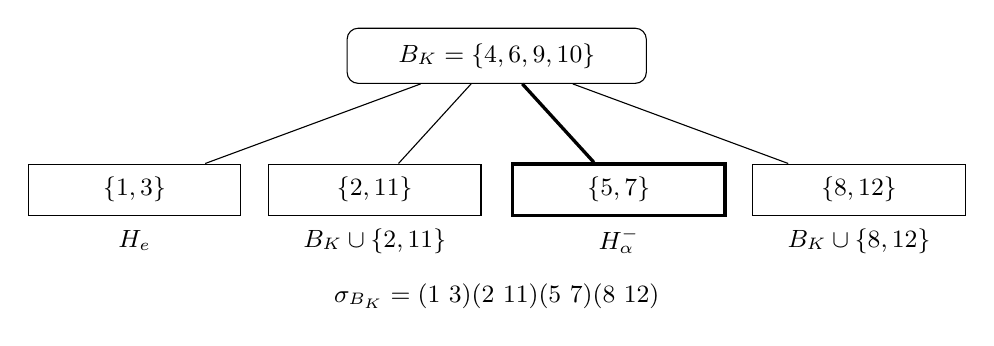
\begin{tikzpicture}[x=1cm,y=1cm, every node/.style={font=\small}]
 \node[draw,rounded corners,minimum width=3.8cm,minimum height=.7cm]
  (b) at (0,0) {$B_K=\{4,6,9,10\}$};
 \node[draw,minimum width=2.7cm,minimum height=.65cm]
  (p1) at (-4.6,-1.7) {$\{1,3\}$};
 \node[draw,minimum width=2.7cm,minimum height=.65cm]
  (p2) at (-1.55,-1.7) {$\{2,11\}$};
 \node[draw,very thick,minimum width=2.7cm,minimum height=.65cm]
  (p3) at (1.55,-1.7) {$\{5,7\}$};
 \node[draw,minimum width=2.7cm,minimum height=.65cm]
  (p4) at (4.6,-1.7) {$\{8,12\}$};
 \draw (b) -- (p1); \draw (b) -- (p2);
 \draw[very thick] (b) -- (p3); \draw (b) -- (p4);
 \node at (-4.6,-2.35) {$H_e$};
 \node at (-1.55,-2.35) {$B_K\cup\{2,11\}$};
 \node at (1.55,-2.35) {$H^-_\alpha$};
 \node at (4.6,-2.35) {$B_K\cup\{8,12\}$};
 \node at (0,-3.05)
  {$\sigma_{B_K}=(1\ 3)(2\ 11)(5\ 7)(8\ 12)$};
\end{tikzpicture}
\caption{L'étoile concrète du drapeau dodécaphasique. Chaque ligne
indique l'union du quadruplet central avec la paire à son extrémité ; la
ligne épaisse signale l'hexade également sélectionnée par les signes
antérieurs à la retenue de $\alpha$. Les quatre paires épuisent les huit
positions extérieures.}
\label{x_reciprocidad:exc:fig-estrella}
\end{figure}

\begin{proposition}[La famille des étoiles]
\label{x_reciprocidad:exc:m12}
Les $\binom{12}4=495$ permutations $\sigma_B$ préservent $\mathcal H$.
Le groupe qu'elles engendrent est d'ordre $95040$ et est le groupe de Mathieu
$M_{12}$ dans son action sur le petit système de Witt.
\end{proposition}

\begin{proof}
L'affirmation de préservation est une vérification finie sur les
$132$ hexades de \eqref{x_reciprocidad:exc:codigo} : pour chaque tétrade, on construit
les quatre pétales et l'on vérifie
$\{\sigma_B(H):H\in\mathcal H\}=\mathcal H$.
La clôture par composition de ces permutations produit $95040$
éléments. Dans l'énumération lexicographique, il suffit d'ajouter successivement
six étoiles qui ne sont pas encore contenues dans le groupe ; les ordres intermédiaires
sont $2,6,18,360,7920,95040$, et les $495$ étoiles appartiennent au groupe
final. La procédure, les six permutations écrites au moyen de leurs
listes d'images et la récurrence de clôture sont développées dans
\ref{iv:iv:apendice-estrellas}. Enfin, on applique la reconnaissance
du groupe d'automorphismes de $S(5,6,12)$ comme $M_{12}$, dont l'ordre est
$12\cdot11\cdot10\cdot9\cdot8=95040$.
\end{proof}

Une étoile individuelle engendre un groupe cyclique d'ordre deux. Elle
n'engendre pas à elle seule $M_{12}$, et encore moins le Monstre. L'
existence de $495$ générateurs d'un groupe de permutations ne prouve pas non plus que
chacun soit le transport d'un lacet spécifique du TPK. Cette affirmation
requiert l'application de lacets correspondante ; le résultat établi ici
est l'action d'incidence finie.

\begin{remark}[L'égalité des traces n'identifie pas les opérateurs]
Sur $V_{11}$, une étoile a pour spectre $+1$ avec multiplicité sept
et $-1$ avec multiplicité quatre. Sa trace normalisée est $3/11$.
Un projecteur de rang trois sur le même espace possède également une trace
normalisée $3/11$, mais un spectre $1^3,0^8$. Ils ne sont pas conjugués : leurs
polynômes minimaux et leurs spectres sont différents. L'opérateur d'entrelacement
\eqref{x_reciprocidad:exc:incidencia} transporte des opérateurs définis ; il ne transforme pas
cette coïncidence scalaire en une équivalence d'opérateurs.
\end{remark}

\subsection{Le résidu binaire et les cinq régions de \texorpdfstring{$\pi$}{pi}}
\label{x_reciprocidad:exc:cinco-regiones}

La reconnaissance suivante utilise le code de Golay binaire
étendu $G_{24}$, de paramètres $[24,12,8]_2$. Ses poids sont
$0,8,12,16,24$, et les supports de poids huit forment le plan
$S(5,8,24)$. Nous fixons une dodécade $D$, support d'un mot de poids
douze. Cette donnée et l'isomorphisme d'incidence qui sera déclaré
ci-dessous appartiennent à la carte de réalisation ; ils ne sont pas utilisés pour
générer ni sélectionner les décimales de $\pi$.

\begin{proposition}[Résidu d'une dodécade et élévation d'hexades]
\label{x_reciprocidad:exc:residuo-binario}
L'ensemble
\[
 \mathcal H(D)=
 \{O\cap D: O\text{ est une octade},\ |O\cap D|=6\}
\]
est un système $S(5,6,12)$ sur $D$. Chacune de ses hexades a une unique élévation en une octade. Pour tout quadruplet $B\subset D$, les cinq octades qui le contiennent se répartissent en quatre élévations résiduelles et une unique octade $O_B^\perp$ avec $O_B^\perp\cap D=B$.
\end{proposition}

\begin{proof}
Un quintuplet $A\subset D$ appartient à une unique octade $O$. Si
$j=|O\cap D|$, le mot binaire somme de $O$ et $D$ a pour poids
$20-2j$. Parmi les poids permis, et avec $0\leq j\leq8$, seuls
$j=2,4,6$ sont possibles. Comme $A\subset O\cap D$, on a $j\geq5$
et donc $j=6$. Cela donne l'existence et l'unicité de l'hexade
résiduelle, ainsi que l'unicité de son élévation en choisissant cinq de ses
points. D'autre part,
\[
 \lambda_4(S(5,8,24))=\frac{\binom{20}1}{\binom41}=5,
 \qquad
 \lambda_4(S(5,6,12))=4.
\]
Les quatre hexades résiduelles sur $B$ donnent quatre octades distinctes. La cinquième ne peut pas couper $D$ en six points, car elle serait une autre hexade résiduelle ; puisqu'elle contient $B$, son intersection est de taille quatre et coïncide avec $B$.
\end{proof}

Une carte $\ell:[12]\to D$ préservant les hexades identifie
$\mathcal H$ à $\mathcal H(D)$. Son existence est la reconnaissance
du plan déjà construit comme le petit plan de Witt ; un choix
concret de $\ell$ fixe le réétiquetage. L'élévation
\[
 \iota_D:\mathcal H\longrightarrow
       \{\text{octades de }G_{24}\},
 \qquad H\longmapsto O\text{ tel que }O\cap D=\ell(H),
\]
est injective parce que l'intersection avec $D$ redonne $\ell(H)$. Cette injectivité a pour domaine les hexades, et non le registre $K$.

La relation avec les cinq régions de $\pi$ conserve des données plus riches
que le nombre cinq. Les émissions et leurs signatures sont :
\begin{center}
\small
\begin{tabular}{@{}crll@{}}
\toprule
Région & Multiplicité & Émission $U_6$ & Signature \\
\midrule
$\perp$ & $432$ & $(501,614,498,169,272,272)$ & $555555$ \\
$++_1$ & $144$ & $(810,923,870,169,272,272)$ & $339555$ \\
$++_2$ & $144$ & $(810,983,810,169,272,272)$ & $393555$ \\
$++_3$ & $144$ & $(870,923,810,169,272,272)$ & $933555$ \\
$--$ & $144$ & $(870,923,810,418,674,521)$ & $933717$ \\
\bottomrule
\end{tabular}
\end{center}
Dans chaque bloc décimal de trois chiffres, la signature utilise la différence
modulaire des deux premiers chiffres. Les cinq émissions ont le
même mot tritique visible $w_\pi=010211$, mais pas la même
généalogie régionale. Les trois régions positives conservent la queue
$169|272|272$ ; la région négative la remplace par $418|674|521$ ;
la région transversale a une signature constante et une multiplicité supérieure.

L'extension marquée de la carte régionale envoie la région transversale sur $O_{\ell(B_K)}^\perp$, la négative sur $\iota_D(H^-_\alpha)$ et les trois positives sur les trois autres élévations de l'étoile. On réalise ainsi la partition $4+1$ des cinq octades sur $\ell(B_K)$. La correspondance individuelle entre les trois noms positifs et les trois pétales restants exige un ordre de carte ; l'incidence ne la détermine pas sans cette donnée. L'affirmation précise est donc une correspondance marquée de régions, compatible avec leurs rôles et avec le drapeau, et non une bijection canonique déduite du cardinal cinq.

L'identité $432+4\cdot144=1008$ conserve les multiplicités
régionales. On a aussi $1008=36\cdot28$ et une octade possède
$\binom82=28$ paires. Ces égalités sont des contrôles arithmétiques de
catalogue, et non des substituts de l'application $\iota_D$ ni de la carte régionale.


% BEGIN OWNER /Users/ruben/Documents/New project/output/EXTREMA_MEDIA_RAZON_RECIPROCIDAD_ES_EN_20260918/ARTICULO/ES/source/sections/estrella_pentadica_recuperada.tex
\subsubsection{Représentation pentadique de la microfibre et de son incidence}
\label{x_reciprocidad:pi-estrella:desarrollo}

La disposition des cinq régions permet de visualiser simultanément
l'unité du quotient ternaire et la différenciation conservée par le
catalogue. L'application pertinente est la restriction
\[
 \Psi\big|_{\mathscr R_\pi^{\rm micro}}:
 \mathscr R_\pi^{\rm micro}\longrightarrow\{010211\},
 \qquad \Psi(U)=(-U)\bmod3.
\]
Ses cinq antécédents sont les vecteurs \(U_6\) du tableau précédent. La figure \ref{x_reciprocidad:pi-estrella:figura} récupère leur organisation radiale, en conservant l'ordre de carte, les signatures et les multiplicités du catalogue (équation~\eqref{x_reciprocidad:eq:palabras-regionales}).


% BEGIN OWNER /Users/ruben/Documents/New project/output/EXTREMA_MEDIA_RAZON_RECIPROCIDAD_ES_EN_20260918/ARTICULO/ES/source/figures/estrella_cinco_regiones.tex
% Orden de carta y datos recuperados de fig_cinco_regiones_pi.tex.
\begin{figure}[H]
\centering
\begin{tikzpicture}[x=1cm,y=1cm,font=\small,>=Latex]
 \coordinate (a) at (90:2.2);
 \coordinate (b) at (18:2.2);
 \coordinate (c) at (-54:2.2);
 \coordinate (d) at (-126:2.2);
 \coordinate (e) at (162:2.2);
 \draw[black!35,line width=.45pt]
    (a)--(c)--(e)--(b)--(d)--cycle;
 \node[draw,fill=white,circle,minimum size=1.6cm,align=center,
    inner sep=3pt] (z) at (0,0) {$w_\pi$\\$010211$};
 \foreach \v in {a,b,c,d,e}{
    \fill (\v) circle (2pt);
    \draw[->,line width=.6pt] (\v)--(z);
 }
 \node[above=3mm,align=center] at (a)
   {$U_\pi^\perp$\\$555555$\\multiplicidad $432$};
 \node[right=3mm,align=left] at (b)
   {$U_{\pi,1}^{++}$\\$339555$\\multiplicidad $144$};
 \node[below right=2mm and 1mm,align=left] at (c)
   {$U_{\pi,2}^{++}$\\$393555$\\multiplicidad $144$};
 \node[below left=2mm and 1mm,align=right] at (d)
   {$U_{\pi,3}^{++}$\\$933555$\\multiplicidad $144$};
 \node[left=3mm,align=right] at (e)
   {$U_\pi^{--}$\\$933717$\\multiplicidad $144$};
 \node[align=center,font=\footnotesize] at (0,-3.55)
   {$1_\perp+3_{++}+1_{--}$\qquad $432+4\cdot144=1008$};
\end{tikzpicture}
\caption{Les cinq régions de \(\pi\) selon une disposition pentadique.
Chaque position conserve sa signature multiplicative et sa multiplicité ;
les flèches radiales représentent la projection commune
\(\Psi(U)=010211\). Le contour étoilé organise les cinq
positions de la carte. Leur réalisation dans les cinq octades de Witt
s'effectue au moyen de l'alignement régional et de la décomposition
\(4+1\) exposée dans le texte.}
\label{x_reciprocidad:pi-estrella:figura}
\end{figure}

% END OWNER


La projection sur le centre identifie les cinq images ternaires ; le
registre des positions extérieures retient l'information régionale
qui rend possible la réalisation d'incidence. La distribution
\(1_\perp+3_{++}+1_{--}\) spécifie une région transversale, trois
régions positives et une négative. Leurs poids normalisés sont
\(3/7\) et \(1/7\) pour chacune des quatre autres : la
multiplicité transversale est triple, alors même que les cinq images par
\(\Psi\) coïncident.

\Needspace{11\baselineskip}
Le lien avec l'étoile de Witt se formule au moyen du drapeau
\(B_K\subset H^-_\alpha\), de l'alignement \(\ell\) et du
relèvement \(\iota_D\) déjà construits. Les cinq positions régionales
se réalisent dans les cinq octades sur \(\ell(B_K)\) :
\[
\begin{aligned}
 U_\pi^\perp&\longmapsto O^\perp_{\ell(B_K)},\\
 U_\pi^{--}&\longmapsto\iota_D(H^-_\alpha),\\
 \{U_{\pi,1}^{++},U_{\pi,2}^{++},U_{\pi,3}^{++}\}
 &\longmapsto
 \{\iota_D(B_K\cup P):P\in\mathcal P_+\},\\
 \mathcal P_+&=\bigl\{\{1,3\},\{2,11\},\{8,12\}\bigr\}.
\end{aligned}
\]
L'attribution des trois positions positives aux trois paires
s'effectue dans une carte ordonnée. La ligne transversale et la ligne négative
sont distinguées par leurs prédicats régionaux et par le drapeau.

Les deux figures s'articulent ainsi : la figure
\ref{x_reciprocidad:exc:fig-estrella} montre les quatre hexades du petit plan
de Witt sur \(B_K\) ; la figure \ref{x_reciprocidad:pi-estrella:figura} montre
les cinq régions qui, sous l'alignement, occupent les quatre octades
résiduelles et l'octade transversale du plan binaire. La loi
\(4+1\), démontrée dans la proposition
\ref{x_reciprocidad:exc:residuo-binario}, spécifie le changement d'incidence. Dans cette
composition, \(K\) détermine la tétrade marquée et la signature de
\(\alpha\) distingue l'une de ses hexades. Les régions conservent,
outre leur valeur ternaire commune, la structure nécessaire à ce
transport vers la réalisation exceptionnelle.

% END OWNER


\subsection{Du code ternaire au réseau de Niemeier}
\label{x_reciprocidad:exc:niemeier}

Le passage à la dimension vingt-quatre ne nécessite pas de parcourir d'abord le
code binaire. Il s'effectue directement à partir de $C_W$ par recollement des
discriminants. On distingue ainsi deux prolongations compatibles :
l'une conserve le résidu $W_{12}\subset W_{24}$ ; l'autre construit le
réseau sur lequel sera réalisée l'algèbre d'opérateurs de vertex.

Soit $A_2=\mathbb Z a_1\oplus\mathbb Z a_2$ de matrice de Gram
\[
 \begin{pmatrix}2&-1\\-1&2\end{pmatrix},
 \qquad \rho=a_1+a_2,\qquad \rho^2=2.
\]
Nous représentons les trois classes de $A_2^*/A_2$ par
\[
 \varpi_0=0,\qquad
 \varpi_1=\frac{2a_1+a_2}{3},\qquad
 \varpi_2=\frac{a_1+2a_2}{3}.
\]
L'application $j\mapsto\varpi_j+A_2$ identifie additivement
$\mathbb F_3$ à ce discriminant. Pour $c\in C_W$, nous écrivons
$\phi(c)=(\varpi_{c_1},\ldots,\varpi_{c_{12}})$ et définissons
\begin{equation}
 N(C_W)=\bigcup_{c\in C_W}\bigl(A_2^{12}+\phi(c)\bigr).
 \label{x_reciprocidad:exc:niemeier-def}
\end{equation}

\begin{theorem}[Recollement ternaire]
\label{x_reciprocidad:exc:niemeier-teorema}
L'objet \eqref{x_reciprocidad:exc:niemeier-def} est un réseau positif, pair et
unimodulaire de rang $24$. Son système de racines est exactement
$A_2^{12}$ ; il est donc reconnu comme le réseau de Niemeier ayant
ce système de racines.
\end{theorem}

\begin{proof}
La linéarité du code rend l'union de classes stable par addition. L'auto-orthogonalité annule l'accouplement discriminant : celui-ci est un multiple de $c\cdot d/3$ modulo $\mathbb Z$. Le réseau est donc entier. La norme d'une classe de recollement est $2\operatorname{wt}(c)/3$ modulo $2\mathbb Z$. Les poids de \eqref{x_reciprocidad:exc:enumerador} sont des multiples de trois, de sorte qu'il est pair.

L'indice de $A_2^{12}$ dans $N(C_W)$ est $|C_W|=3^6$. En conséquence,
\[
 \det N(C_W)=\frac{3^{12}}{(3^6)^2}=1.
\]
La positivité procède de la somme orthogonale des douze métriques $A_2$.
Dans une classe non nulle de $A_2^*/A_2$, la norme minimale est $2/3$ ;
tout mot non nul possède au moins six positions non nulles.
Par conséquent, un vecteur d'une classe de recollement non triviale a une norme
au moins égale à $6\cdot2/3=4$. Aucune racine de norme deux n'apparaît hors de
$A_2^{12}$. À l'intérieur de celui-ci, les racines sont précisément celles de ses
douze composantes.
\end{proof}

\subsection{Sélection par incidence du voisin unimodulaire sans racines}
\label{x_reciprocidad:exc:leech}


% BEGIN OWNER /Users/ruben/Documents/New project/output/EXTREMA_MEDIA_RAZON_RECIPROCIDAD_ES_EN_20260918/ARTICULO/ES/source/sections/incidencia_reticulo.tex
\paragraph{De l'origine incidencielle à la modification réticulaire.}
\label{x_reciprocidad:inc-ampl-reticulo}
Le drapeau marqué détermine une position au moyen d'une opération
ensembliste équivariante :
\[
 o_*=(H_e\cap H_\varphi)
       \setminus(H^-_\alpha\cup H_{\rm APP})=\{1\}.
\]
Sa fonction consiste à distinguer une composante parmi les douze qui
interviennent dans la réalisation réticulaire. Le code ternaire complet
agit comme code de recollement dans le module discriminant
$(A_2^*/A_2)^{12}$. Sa préimage définit $N(C_W)$, et
l'autodualité, les poids et la distance du code se traduisent,
respectivement, en propriétés d'intégralité et de déterminant, de parité
et en bornes de norme des classes de recollement. L'information symbolique
du code remplit ici une fonction que le support isolé ne remplit plus.

La métrique $A_2$ et la chambre radiale positive sont fixées dans le développement
réticulaire. À l'intérieur de cette chambre, la congruence nécessaire pour un voisin
pair d'indice trois possède douze réalisations de norme minimale $54$,
permutées par le changement de composante distinguée. L'origine $o_*$
sélectionne
\[
 v_\alpha=4\rho_1+\rho_2+\cdots+\rho_{12},\qquad
 v_\alpha^2=2(4^2+11)=54.
\]
Le coefficient $4$ appartient à cette solution de la congruence dans la
chambre déclarée. L'indice $\alpha$ enregistre la provenance
incidencielle de la sélection : son contenu est le repère qui est intervenu dans
la clôture et qui individualise à présent une direction réticulaire.

L'appariement avec $v_\alpha$ détermine le sous-réseau
$N_{\alpha,0}$ d'indice trois, et l'adjonction de la classe
$v_\alpha/3$ produit le voisin $N_\alpha$ de
\eqref{x_reciprocidad:exc:vecino}. Cette modification conserve le rang et rétablit
l'unimodularité et la parité ; la sélection par congruence élimine les racines
antérieures, et les bornes locales excluent les racines dans les nouvelles classes.
L'identification à Leech intervient après ces vérifications. La
réalisation binaire des cinq régions et cette construction réticulaire
sont deux prolongements du repère commun : la seconde reçoit directement
le code ternaire comme donnée de recollement.


% END OWNER


L'étiquette $o_*=1$ du drapeau se réalise maintenant comme l'une des
douze composantes $A_2$. Cette opération déclare la métrique précédente et
la chambre radiale positive
\[
 v(a)=\sum_{i=1}^{12}a_i\rho_i,
 \qquad a_i=1+3b_i,\quad b_i\in\mathbb Z_{\geq0}.
\]
L'exigence de parité du voisin d'indice trois est $v(a)^2\equiv0\pmod{18}$. Puisque
\[
 v(a)^2=2\sum_i(1+3b_i)^2,
\]
cette congruence équivaut à $\sum_i b_i\equiv1\pmod3$. La plus petite
valeur de la norme dans la chambre s'obtient avec un unique $b_i=1$ et
tous les autres nuls ; elle vaut $54$. L'origine marquée sélectionne
\begin{equation}
 v_\alpha=4\rho_1+\rho_2+\cdots+\rho_{12},
 \qquad v_\alpha^2=54.
 \label{x_reciprocidad:exc:vector}
\end{equation}
Le mot ``plus petit'' se rapporte à cette chambre positive. Il n'affirme pas la minimalité dans toute la classe résiduelle : le vecteur $(a_1-2a_2,\rho,\ldots,\rho)$ représente la même classe modulo trois et a pour norme $14+11\cdot2=36$. La restriction de chambre fait partie des données de la construction, et n'est pas une conclusion que l'on puisse omettre.

Soit $N=N(C_W)$. Nous définissons
\begin{equation}
 N_{\alpha,0}=\{x\in N:\langle x,v_\alpha\rangle\equiv0\pmod3\},
 \qquad
 N_\alpha=N_{\alpha,0}+\mathbb Z\frac{v_\alpha}{3}.
 \label{x_reciprocidad:exc:vecino}
\end{equation}

\begin{theorem}[Voisin de Leech déterminé par le drapeau marqué]
\label{x_reciprocidad:exc:teorema-leech}
Avec la métrique et la chambre déclarées, $N_\alpha$ est un réseau
positif, pair et unimodulaire de rang $24$, sans vecteurs de norme deux.
D'après le théorème de classification correspondant, il est isométrique au
réseau de Leech $\Lambda_{24}$.
\end{theorem}

\begin{proof}
Le caractère $x\mapsto\langle x,v_\alpha\rangle\bmod3$ est non nul :
une racine simple d'une composante s'apparie avec $a_i\rho_i$ en
$a_i\equiv1\pmod3$. Par conséquent, $[N:N_{\alpha,0}]=3$ et
$\det N_{\alpha,0}=9$. De plus,
$v_\alpha/3\in N_{\alpha,0}^*$ et $v_\alpha\in N_{\alpha,0}$.
Si $v_\alpha/3$ appartenait à $N$, l'intégralité de $N$ rendrait
tous les appariements avec $v_\alpha$ divisibles par trois,
ce qui contredirait le caractère non nul. La classe de $v_\alpha/3$ est
donc d'ordre trois. On en déduit
\[
 [N_\alpha:N_{\alpha,0}]=3,
 \qquad \det N_\alpha=9/3^2=1.
\]
L'extension est entière, et pour $x\in N_{\alpha,0}$,
\[
 \left(x+m\frac{v_\alpha}{3}\right)^2
   =x^2+2m\frac{\langle x,v_\alpha\rangle}{3}+6m^2
   \in2\mathbb Z.
\]
Elle est donc paire.

Il reste à exclure les racines, ce qui est l'étape décisive. Les racines de $N$ appartiennent à $A_2^{12}$. Leurs accouplements avec $v_\alpha$ sont congrus à $\pm1$ ou à $\pm2$ modulo trois ; aucune n'appartient à $N_{\alpha,0}$. Pour les deux autres classes du voisin, chaque composante appartient à l'une des classes locales
\[
 A_2+\varpi_j\pm\rho/3,\qquad j=0,1,2.
\]
Comme $4\rho/3\equiv\rho/3\pmod{A_2}$, cette description vaut
également dans la composante distinguée. En écrivant un vecteur local
sous la forme $(u a_1+v a_2)/3$, sa norme est
$2(u^2-uv+v^2)/9$. Les six classes précédentes ont des résidus non
nuls et un minimum $2/9$ : les représentants de forme quadratique minimale
sont $(\pm1,0),(0,\pm1),(1,1),(-1,-1)$ dans les résidus appropriés.
Un vecteur d'une classe nouvelle a donc une norme au moins égale à
$12\cdot2/9=8/3>2$. Aucune des trois classes ne contient de racines.
La classification des réseaux pairs unimodulaires positifs de
rang vingt-quatre identifie l'unique cas sans racines à
$\Lambda_{24}$.
\end{proof}

L'argument ne reconnaît pas Leech par une coïncidence de dimension.
Il construit le recollement, prouve l'intégralité, la parité et le déterminant, et
élimine les racines au moyen d'une borne locale. Ce n'est qu'ensuite qu'il applique le
théorème de classification. La dépendance à l'égard de $\alpha$ est conservée dans
le drapeau qui sélectionne $o_*$ et dans le vecteur \eqref{x_reciprocidad:exc:vector} ;
on ne transforme pas la valeur scalaire de la constante en une longueur du
réseau.

\subsection{L'algèbre d'opérateurs de vertex et le Monstre}
\label{x_reciprocidad:exc:voa}

Soit $\Lambda=N_\alpha$, déjà reconnu comme le réseau de Leech. L'étape suivante utilise son réseau entier, et non un développement décimal. La construction de l'algèbre d'opérateurs de vertex de réseau s'écrit
\[
 V_\Lambda=M(1)\otimes\mathbb C_\varepsilon[\Lambda].
\]
Ici, $M(1)$ est l'espace des oscillateurs de Heisenberg en rang vingt-quatre ; $\mathbb C_\varepsilon[\Lambda]$ est l'algèbre de groupe tordue par le cocycle de l'extension centrale du réseau. Le cocycle et le relèvement des isométries font partie de la construction : une somme vectorielle nue ne détermine pas les produits de vertex.

La négation $\lambda\mapsto-\lambda$ admet le relèvement standard
$\theta$. Avec son module tordu et le choix de parité compatible,
la construction de Frenkel--Lepowsky--Meurman produit
\begin{equation}
 V^\natural_{\rm HMT}
   =V_\Lambda^+\oplus(V_\Lambda^T)^+.
 \label{x_reciprocidad:exc:flm}
\end{equation}
Le signe $+$ désigne la partie paire de l'action relevée. L'expression
inclut le produit de vertex de l'orbifold ; elle ne se limite pas à une somme
d'espaces gradués.

\begin{theorem}[Prolongement jusqu'au module Moonshine]
\label{x_reciprocidad:exc:moonshine}
L'algèbre \eqref{x_reciprocidad:exc:flm}, construite sur le voisin
\eqref{x_reciprocidad:exc:vecino}, est une réalisation de l'algèbre Moonshine
$V^\natural$. Elle a une charge centrale $24$, une composante de poids un nulle
et un groupe d'automorphismes isomorphe au Monstre $\mathbb M$. Son caractère
gradué est
\begin{equation}
 \operatorname{Tr}_{V^\natural_{\rm HMT}}q^{L_0-1}
   =J(\tau)=j(\tau)-744
   =q^{-1}+196884q+21493760q^2+\cdots,
 \qquad q=e^{2\pi i\tau}.
 \label{x_reciprocidad:exc:j}
\end{equation}
\end{theorem}

\begin{proof}
Le théorème \ref{x_reciprocidad:exc:teorema-leech} vérifie les hypothèses sur le réseau :
positivité, parité, unimodularité, rang vingt-quatre et absence de
racines. On applique alors la construction et le théorème de
Frenkel--Lepowsky--Meurman pour le réseau de Leech. Ceux-ci identifient
l'orbifold à $V^\natural$, établissent son caractère et son groupe d'
automorphismes. La composition du drapeau, du voisin et du foncteur
de construction de VOA donne la réalisation indiquée ici. Le groupe ne se déduit
pas du coefficient $196884$.
\end{proof}

Le théorème utilisé est une reconnaissance classique ultérieure dont les hypothèses sont vérifiées, et non une nouvelle démonstration dans cet article de la construction FLM \cite{x_reciprocidad:flm}. En outre, la notation $q=e^{2\pi i\tau}$ est la variable conventionnelle de Fourier employée pour reconnaître le caractère. Elle n'introduit ni $\pi$ ni $e$ comme entrées du générateur coinductif qui les a déjà déterminés.

Une partie du mécanisme de trace peut être observée avant l'orbifold.
Seul le vecteur nul du réseau est fixé par la négation ; chaque
oscillateur contribue avec un signe alterné. D'où
\[
 \operatorname{Tr}_{V_\Lambda}\theta q^{L_0-1}
   =t_2(\tau)
   :=q^{-1}\prod_{n\geq1}(1+q^n)^{-24}.
\]
Cette trace dans l'algèbre de réseau ne doit pas être confondue avec le
caractère sans insertion de $V^\natural$. Elle n'identifie pas non plus à elle
seule une classe de conjugaison du Monstre : l'espace, l'insertion
et le relèvement doivent être spécifiés avant de comparer les fonctions.


% BEGIN OWNER /Users/ruben/Documents/New project/output/EXTREMA_MEDIA_RAZON_RECIPROCIDAD_ES_EN_20260918/ARTICULO/ES/source/sections/incidencia_automorfismos.tex
\paragraph{Graduation, unité et automorphismes.}
\label{x_reciprocidad:inc-ampl-automorfismos}
La construction de Frenkel--Lepowsky--Meurman s'applique au réseau
$N_\alpha$ une fois ses propriétés vérifiées. Elle incorpore l'espace
des oscillateurs, l'extension centrale du réseau, le produit de vertex
et le secteur tordu par le relèvement de la négation. Le résultat est
l'algèbre $V^\natural_{\rm HMT}$ de \eqref{x_reciprocidad:exc:flm}, dont le groupe
d'automorphismes est isomorphe au Monstre. Son domaine d'action est ainsi
fixé par une structure algébrique munie d'une graduation et d'un produit. Le théorème
de Moonshine de Borcherds détermine ensuite les traces graduées
avec insertion de ces automorphismes \cite{x_reciprocidad:flm,x_reciprocidad:borcherds}.

L'unité acquiert à ce niveau une réalisation précise : la composante
de poids zéro est la droite du vide et fournit le coefficient $1$ de
$q^{-1}$ dans le caractère gradué. Au niveau cylindrique, les
applications de raffinement conservent la fonction constante par
précomposition. Chaque assertion de conservation possède donc son
objet et son application. Le développement des preuves rend visible cette
continuité de construction, depuis les opérations arithmétiques et la
mémoire jusqu'à l'incidence, à la métrique et aux produits de vertex.

Cette articulation situe $K$ et la clôture de $\alpha$ dans l'argument
principal. $K$ conserve de manière réversible une coordonnée entière de
l'histoire ; la normalisation de $\alpha$ compose les registres régionaux
avec cette coordonnée ; la configuration signée détermine un drapeau ; et
le drapeau marqué sélectionne la modification réticulaire sur laquelle se
réalise Moonshine. Les démonstrations suivantes développent ces
applications, en distinguant les équivalences réversibles, les quotients
d'information et les réalisations qui ajoutent une métrique ou une structure
algébrique. Ainsi s'exprime une relation démontrable entre structure,
équation et valeur, en conservant l'attribution de chaque construction et la
portée de ses théorèmes.

% END OWNER



% BEGIN OWNER /Users/ruben/Documents/New project/output/EXTREMA_MEDIA_RAZON_RECIPROCIDAD_ES_EN_20260918/ARTICULO/ES/source/sections/fibras_app_witt.tex
\subsection{Construction à partir de l’état des douze fibres cyclotomiques}
\label{x_reciprocidad:nuclear:fibras-app-witt}
Sur les marques d’APP, la multiplication \(a:r\mapsto4r\) dans
\(\ZZ/9\ZZ\) satisfait \(a^3=1\). Les feuillets vérifient
\[
 S(ax,ay)=aS(x,y),\qquad P(ax,ay)=a^{-1}P(x,y),
\]
puisque \(16\equiv7\equiv4^{-1}\pmod9\). Les orbites unitaires
ordonnées sont \(\mathcal O_0=(1,4,7)\), \(\mathcal O_1=(2,8,5)\).
Dans chacune, le module d’augmentation
\(A(\mathcal O)=\ker(\ZZ[\mathcal O]\xrightarrow{\sum}\ZZ)\)
hérite du produit qui rend les \(e_r\) orthonormaux. Dans la base
\(b_1=e_r-e_{4r}\), \(b_2=e_{4r}-e_{7r}\), ses matrices sont
\[
 G_{A_2}=\begin{pmatrix}2&-1\\-1&2\end{pmatrix},\qquad
 C=\begin{pmatrix}0&-1\\1&-1\end{pmatrix},\qquad
 C^{\mathsf T}G_{A_2}C=G_{A_2}.
\]
La forme réticulaire provient donc des orbites des marques. Pour les paires \((1,2),(2,3),(3,1)\) et les feuillets \(\mu\in\{\Sigma,\Pi\}\), on obtient
\[
 W_{\APP}=\bigoplus_{(i,j)}\bigoplus_\mu\bigoplus_{\varepsilon=0}^1
 A(\mathcal O_\varepsilon),\qquad
 \ell^\Sigma_{ij}(x)=x_i+x_j,\quad
 \ell^\Pi_{ij}(x)=x_ix_j\pmod9.
\]
Chaque terme conserve la paire, le feuillet et l'orbite. L'application d'état est
\[
 \Psi:(\ZZ/9\ZZ)^3\longrightarrow W_{\APP},\qquad
 \Psi(x)_{ij,\mu,\varepsilon}=\beta_\varepsilon(\ell^\mu_{ij}(x)),
 \quad
 \beta_\varepsilon(r)=
 \begin{cases}e_r-e_{4r},&r\in\mathcal O_\varepsilon,\\0,&r\notin\mathcal O_\varepsilon.
 \end{cases}
\]
\begin{proposition}[Équivariance et rang du module d’état]
\label{x_reciprocidad:nuclear:psi-rango}
L’action de \(C\) dans les six fibres additives et de \(C^{-1}\) dans
les six fibres multiplicatives vérifie \(\Psi(ax)=\rho(a)\Psi(x)\).
Les images engendrent \(W_{\APP}\otimes\QQ\), de dimension vingt-quatre.
\end{proposition}
\begin{proof}
Les identités des feuillets et \(\beta(4r)=C\beta(r)\) prouvent
l’équivariance. Pour le rang, on ordonne les coordonnées par les trois
couples indiqués, par \(\Sigma,\Pi\), par \(\mathcal O_0,\mathcal O_1\)
et par \(b_1,b_2\). Dans chaque orbite, \(\beta\) prend successivement
\((1,0),(0,1),(-1,-1)\). La matrice des images de ces états,
lus par lignes, a pour déterminant \(9\) :
\[
\begin{array}{rrrr}
(0,0,1)&(0,0,2)&(0,0,4)&(0,0,5)\\
(0,1,0)&(0,1,1)&(0,1,2)&(0,1,3)\\
(0,1,4)&(0,1,5)&(0,1,6)&(0,2,0)\\
(0,2,2)&(0,2,3)&(0,4,0)&(0,5,0)\\
(1,0,1)&(1,0,2)&(1,0,4)&(1,0,5)\\
(1,1,0)&(1,2,0)&(1,4,0)&(1,5,0).
\end{array}
\]
L'élimination successive, en réduisant chaque ligne par les précédentes et en normalisant son premier coefficient non nul, donne les colonnes pivots numérotées à partir de zéro
\[
\begin{split}
&(8,10,9,11,0,12,14,16,13,15,17,2,\\
&\hspace{2em}18,19,1,3,20,22,21,23,4,6,5,7)
\end{split}
\]
et pivots
\[
(1,1,1,-1,1,1,1,1,1,-1,3,1,1,3,1,-1,1,1,1,-1,1,1,1,-1).
\]
Leur produit, multiplié par le signe de la permutation des colonnes,
est \(9\). Le mineur inversible atteste le rang total.
\end{proof}

\subsection{Alignement dodécaphasique avec les positions de Witt}
\label{x_reciprocidad:nuclear:alineamiento-witt}
L'indice de la paire est \(i\in\ZZ/3\ZZ\), celui du feuillet \(\mu\in\{0,1\}\) et celui de l'orbite \(\varepsilon\in\{0,1\}\). L'origine dodécaphasique étant fixée, \(\lambda(i,\mu,\varepsilon)
=4i+2\mu+\varepsilon\pmod{12}\) est bijective : les quatre valeurs de chaque \(i\) forment un bloc et les trois blocs sont disjoints. Soit \(R=\left(\begin{smallmatrix}0&1\\1&0\end{smallmatrix}\right)\).
La multiplication prouve \(RCR=C^{-1}\) et
\(R^{\mathsf T}G_{A_2}R=G_{A_2}\). Pour les trivialisations
\(\iota_b\) et les repères \(P_b\) transportés conjointement avec
l’incidence de Witt, nous posons
\[
g_b=\iota_b^{-1}P_bCP_b^{-1}\iota_b,\qquad
T_{i\mu\varepsilon}=\iota_{\lambda(i,\mu,\varepsilon)}^{-1}
P_{\lambda(i,\mu,\varepsilon)}R^\mu.
\]
Alors
\[
g_{\lambda(i,\mu,\varepsilon)}T_{i\mu\varepsilon}
=T_{i\mu\varepsilon}C^{(-1)^\mu}.
\]
La somme directe est un isomorphisme \(C_3\)-équivariant entre les douze
fibres d’état et les douze positions réticulaires. Elle conserve couple,
feuillet, orbite et forme sous le transport simultané de l’origine,
de l’ordre et de l’orientation. Ces données demeurent dans le recollement réticulaire
et le passage au voisin construits ci-dessous.

% END OWNER


% BEGIN OWNER /Users/ruben/Documents/New project/output/EXTREMA_MEDIA_RAZON_RECIPROCIDAD_ES_EN_20260918/ARTICULO/ES/source/sections/moonshine_comparacion.tex
% Incorporación aditiva para el Artículo I; no modifica la fuente anterior.
% RESULTADO_RECUPERADO: integral, capítulo 22, propietario extenso
% colaboracion/partes_i_ii/source/base_residencias/
% capitulo_22_c20_lineas_2613_3270.tex, líneas 176--576.
% Equivalencia 2/3: public/residencias/capitulo_22_voa_leech_moonshine.tex,
% líneas 55--127. Orden dos y Fricke: hmt/15d_voa_moonshine_orden_dos_rev11.tex.
% Prerrequisitos residentes en I: código C_W, matriz A_W, N(A_2^12),
% origen o_*, vector v_alpha de norma54, N_alpha reconocido como Leech,
% VOA reticular y presentación FLM de las secciones precedentes.
% Bibliografía nueva: chenlamshimakura2016, abelamyamada2017,
% kmconwaynorton1979 (bibitems listos para incorporar al final de este archivo).

\subsection{Orientation ternaire du voisin de Leech}
\label{x_reciprocidad:km:orden-tres-reticular}

La présentation d’ordre deux construite précédemment utilise la négation
du réseau de Leech. Le même réseau, obtenu à partir de l’incidence marquée
par \(K\) et du support dodécaphasique de \(\alpha\), admet une seconde
présentation compatible avec le caractère ternaire de la construction.
Pour expliciter cette continuité, on conserve le recollement, on construit
son isométrie d’ordre trois et l’on vérifie qu’elle préserve le voisin déjà
sélectionné. Cette étape ne requiert pas d’altérer \(K\), sa lecture rationnelle ni
la définition préalable de \(\alpha\). On développe ici le prolongement d’ordre trois, y compris les opérations
réticulaires et les conditions précises des théorèmes classiques utilisés.

Nous travaillons dans la base des racines simples de chaque facteur \(A_2\), avec
\begin{equation}
 B_2=\begin{pmatrix}2&-1\\-1&2\end{pmatrix},\qquad
 \mathsf C=\begin{pmatrix}0&-1\\1&-1\end{pmatrix},\qquad
 \mathsf R=\begin{pmatrix}0&1\\1&0\end{pmatrix},\qquad
 \rho=\begin{pmatrix}1\\1\end{pmatrix}.
 \label{x_reciprocidad:km:coxeter-reflexion}
\end{equation}
La multiplication donne
\[
 \mathsf C^3=I_2,\quad
 \mathsf C^2+\mathsf C+I_2=0,\quad
 \mathsf C^{\mathsf T}B_2\mathsf C=B_2,\quad
 \mathsf R\mathsf C\mathsf R=\mathsf C^{-1},\quad
 \mathsf R^{\mathsf T}B_2\mathsf R=B_2.
\]
Ces identités fixent aussi bien la métrique que l'orientation de l'action. Dans le discriminant \(A_2^*/A_2\cong\mathbb F_3\), nous prenons pour générateur la classe de \(\varpi=(2,1)^{\mathsf T}/3\). On a \(\mathsf C\varpi-\varpi=(-1,0)^{\mathsf T}\), de sorte que \(\mathsf C\) agit trivialement sur le discriminant ; la réflexion \(\mathsf R\) change son signe.

La matrice de Paley--Witt déjà construite produit un élément de support
complet par l'opération suivante :
\begin{equation}
 \begin{gathered}
 q_*=(1,1,1,1,1,1),\qquad q_*A_W=(2,1,1,1,1,1),\\
 c_*=(q_*,q_*A_W)
 =(1,1,1,1,1,1,2,1,1,1,1,1)\in C_W.
 \end{gathered}
 \label{x_reciprocidad:km:palabra-total}
\end{equation}
Chaque coordonnée de \(c_*\) est non nulle. Pour les douze positions,
nous définissons les cadres et l'isométrie
\begin{equation}
 P_b(c_*)=
 \begin{cases}\mathsf R,&(c_*)_b=1,\\I_2,&(c_*)_b=2,\end{cases}
 \qquad
 g_c=\bigoplus_{b=1}^{12}P_b(c_*)\mathsf C P_b(c_*)^{-1}.
 \label{x_reciprocidad:km:isometria-ternaria}
\end{equation}
Le symbole \(P_b(c_*)\) désigne ici un repère inversible d’un facteur
\(A_2\), et non le projecteur régional \(P_3\).

\begin{proposition}[Isométrie d'ordre trois sur le voisin marqué]
\label{x_reciprocidad:km:estabilidad-vecino}
L'opérateur \(g_c\) est une isométrie d'ordre trois sans vecteurs fixes non nuls. Il préserve le réseau de Niemeier \(N=N(C_W)\) et le voisin \(N_\alpha\) construit dans \eqref{x_reciprocidad:exc:vecino}.
\end{proposition}
\begin{proof}
Chaque bloc de \(g_c\) est \(\mathsf C\) ou \(\mathsf C^{-1}\) ;
son polynôme minimal est \(X^2+X+1\). Cela prouve l'ordre et
l'absence de vecteurs fixes. Les deux blocs agissent trivialement sur le
discriminant, de sorte qu'ils conservent chaque classe de recollement et donc
le réseau \(N\).

Écrivons \(v=v_\alpha=4\rho_{o_*}+\sum_{b\ne o_*}\rho_b\),
avec les cadres et l'origine d'incidence déjà fixés. Ses coefficients
radiaux sont \(a_{o_*}=4\) et \(a_b=1\) pour \(b\ne o_*\).
Tous satisfont \(a_b\equiv1\pmod3\). Dans un facteur,
\[
 (\mathsf C-I_2)\rho=(-2,-1)^{\mathsf T},\qquad
 (\mathsf C^{-1}-I_2)\rho=(-1,-2)^{\mathsf T}.
\]
Après division par trois, leurs classes discriminantes sont respectivement \(2\) et \(1\). En conséquence, les vecteurs
\begin{equation}
 y=\frac{g_cv-v}{3},\qquad z=\frac{g_c^{-1}v-v}{3}
 \label{x_reciprocidad:km:desplazamientos}
\end{equation}
ont pour mots discriminants \(c_*\) et \(-c_*\), tous deux dans
\(C_W\). Par conséquent, \(y,z\in N\). Le produit local est
\[
 \left\langle
 \frac{(\mathsf C^{\pm1}-I_2)a_b\rho}{3},a_b\rho
 \right\rangle=-a_b^2,
\]
et leur somme donne \(\langle y,v\rangle=\langle z,v\rangle=-(16+11)=-27\). Ainsi, \(y,z\in N_0=\{x\in N:\langle x,v\rangle\equiv0\pmod3\}\). Pour \(x\in N_0\),
\[
 \langle g_cx,v\rangle
 =\langle x,g_c^{-1}v\rangle
 =\langle x,v\rangle+3\langle x,z\rangle\equiv0\pmod3.
\]
L'argument appliqué à \(g_c^{-1}\) prouve \(g_cN_0=N_0\).
Enfin, \(g_c(v/3)=v/3+y\) conserve la classe qui engendre
\(N_\alpha=N_0+\mathbb Z(v/3)\). On obtient
\(g_cN_\alpha=N_\alpha\).
\end{proof}

La preuve conserve plus que la dimension du réseau : elle utilise le code de recollement, son orientation, l'origine du drapeau et la congruence du vecteur radial. Ces données expliquent pourquoi la seconde présentation reste liée au registre dodécaphasique dont la construction est partie.

\subsection{Trace ternaire, poids tordu et extension d'ordre trois}
\label{x_reciprocidad:km:orbifold-tres}

Soit \(\Lambda=N_\alpha\) et soit \(\widehat g_c\) le relèvement
standard de \(g_c\) à l'algèbre de réseau
\(V_\Lambda=M(1)\otimes\mathbb C_\varepsilon[\Lambda]\), avec
l'extension centrale et le cocycle déjà déclarés. L'ordre impair permet
de choisir ce relèvement d'ordre trois. Chaque facteur complexe \(A_2\)
apporte les valeurs propres \(\zeta_3\) et \(\zeta_3^2\), où
\(\zeta_3^2+\zeta_3+1=0\).

\begin{proposition}[Trace graduée et type du relèvement]
\label{x_reciprocidad:km:traza-tipo}
Pour \(j=1,2\),
\begin{equation}
 \operatorname{Tr}_{V_\Lambda}
       \bigl(\widehat g_c^{\,j}q^{L_0-1}\bigr)
 =t_3(\tau)
 :=q^{-1}\prod_{n\ge1}(1+q^n+q^{2n})^{-12}.
 \label{x_reciprocidad:km:tres-traza}
\end{equation}
Le poids minimal des modules tordus non triviaux est \(4/3\), et
le relèvement est de type zéro.
\end{proposition}
\begin{proof}
Dans la partie réticulaire de la trace, seul le vecteur nul contribue,
car \(g_c\) et \(g_c^2\) n'ont pas de vecteurs fixes non nuls.
À chaque degré d'oscillateur, la trace des puissances symétriques est l'inverse
du déterminant \(I-g_c^jq^n\). Chaque facteur \(A_2\) contribue
\(1+q^n+q^{2n}\), ce qui démontre \eqref{x_reciprocidad:km:tres-traza}.

La formule du poids du vide tordu pour un automorphisme de réseau d'ordre trois, appliquée aux deux espaces propres de dimension douze, donne
\[
 \rho_{\widehat g_c}
 =\frac{1}{4\cdot3^2}
   \bigl(1\cdot2\cdot12+2\cdot1\cdot12\bigr)=\frac43.
\]
Le type est la classe de \(3^2\rho_{\widehat g_c}=12\) modulo
trois, qui est nulle. La formule de poids est un résultat de la théorie des
modules tordus ; les multiplicités et l'isométrie qui l'alimentent
ont été construites ici.
\end{proof}

\begin{theorem}[Seconde présentation de l'algèbre Moonshine]
\label{x_reciprocidad:km:moonshine-tres}
L'extension cyclique de type zéro
\begin{equation}
 V_{(3)}=\operatorname{Orb}_{\mathbb Z/3}
                 (V_\Lambda,\widehat g_c)
 \label{x_reciprocidad:km:extension-orden3}
\end{equation}
est isomorphe à l'algèbre d'opérateurs de vertex \(V^\natural\).
\end{theorem}
\begin{proof}
Le théorème \ref{x_reciprocidad:exc:teorema-leech} fournit un réseau positif,
pair, unimodulaire, de rang vingt-quatre et sans racines. La
Proposition~\ref{x_reciprocidad:km:estabilidad-vecino} construit sur ce même
réseau une isométrie d'ordre trois sans vecteurs fixes ; la
Proposition~\ref{x_reciprocidad:km:traza-tipo} vérifie le relèvement et son type.
On applique alors le théorème de Chen--Lam--Shimakura sur l'
orbifold d'ordre trois de l'algèbre du réseau de Leech
\cite[Teorema~1.1]{x_reciprocidad:chenlamshimakura2016}. L'identification est également comprise
dans le traitement uniforme d'Abe--Lam--Yamada
\cite[Teorema~4.4 y secciones~2--4]{x_reciprocidad:abelamyamada2017}. Cette application est postérieure à la construction
des données du réseau ; l'égalité des caractères ne remplace pas les
hypothèses du théorème utilisé.
\end{proof}

Pour préciser la symétrie duale, écrivons \(V_{(3)}=W_0\oplus W_1\oplus W_2\), où \(W_i\) est le secteur entier sélectionné dans le module \(\widehat g_c^{\,i}\)-tordu. Le produit satisfait \(Y(W_i,z)W_j\subset W_{i+j\bmod3}((z))\). Par conséquent,
\begin{equation}
 g^\vee|_{W_i}=\zeta_3^i I
 \label{x_reciprocidad:km:dual-ciclico}
\end{equation}
définit un automorphisme d'ordre trois. En effet, le facteur sur un
produit est \(\zeta_3^{i+j}=\zeta_3^i\zeta_3^j\), et le vide et le
vecteur conforme appartiennent à \(W_0\). L'identification classique de
cet automorphisme dans le Monstre est la classe \(3B\), de série
\(T_{3B}=t_3+12\) \cite{x_reciprocidad:kmconwaynorton1979,x_reciprocidad:borcherds}.
Cette normalisation peut être vérifiée dans la construction. Le caractère
du réseau est \(\operatorname{ch}V_\Lambda=J+24\) : son pôle initial
est \(q^{-1}\), son espace de poids un est de dimension 24 et le
caractère modulaire de poids zéro est déterminé par ces données.
Si \(F\) est le caractère du sous-espace fixe et \(H\) celui de chaque
secteur tordu entier, la projection sur les invariants et la conjugaison
des deux secteurs donnent
\[
 F=\frac{J+24+2t_3}{3},\qquad F+2H=J,
 \qquad \operatorname{Tr}g^\vee q^{L_0-1}=F-H=t_3+12.
\]
Son domaine est l'algèbre étendue, tandis que \(\widehat g_c\) agit sur l'algèbre de réseau précédente.

\subsection{Équivalence des présentations d'ordres deux et trois}
\label{x_reciprocidad:km:equivalencia-dos-tres}

Notons
\[
 V_{(2)}=(V_\Lambda)^+\oplus(V_\Lambda^T)^+
\]
la présentation FLM de \eqref{x_reciprocidad:exc:flm}. Les deux présentations conservent le même voisin de Leech comme antécédent. Leurs extensions emploient des automorphismes différents et des produits de vertex déterminés au moyen des données de relèvement respectives.

\begin{theorem}[Équivalence graduée et transport d'automorphismes]
\label{x_reciprocidad:km:equivalencia-voa}
Des isomorphismes d'algèbres d'opérateurs de vertex étant fixés
\[
 \phi_2:V_{(2)}\xrightarrow{\ \cong\ }V^\natural,
 \qquad
 \phi_3:V_{(3)}\xrightarrow{\ \cong\ }V^\natural,
\]
la composition
\begin{equation}
 \Phi_{23}=\phi_2^{-1}\phi_3:
 V_{(3)}\xrightarrow{\ \cong\ }V_{(2)}
 \label{x_reciprocidad:km:Phi23}
\end{equation}
conserve le vide, le vecteur conforme, la graduation et le produit de vertex. La conjugaison par \(\Phi_{23}\) identifie les groupes d'automorphismes et conserve leurs traces graduées.
\end{theorem}
\begin{proof}
La composition des deux isomorphismes préserve les structures
déclarées. En particulier,
\[
 \Phi_{23}Y_{(3)}(a,z)b
 =Y_{(2)}(\Phi_{23}a,z)\Phi_{23}b,
 \qquad
 \Phi_{23}L_0^{(3)}=L_0^{(2)}\Phi_{23}.
\]
Si \(h\) est un automorphisme de \(V_{(3)}\), alors
\(h' =\Phi_{23}h\Phi_{23}^{-1}\) est un automorphisme de
\(V_{(2)}\). L'égalité des traces sur chaque composante homogène
de dimension finie donne
\[
 \operatorname{Tr}_{V_{(3)}}h q^{L_0-1}
 =\operatorname{Tr}_{V_{(2)}}h' q^{L_0-1}.
\]
\end{proof}

Le choix de \(\phi_2\) et \(\phi_3\) fait partie de l'énoncé ;
\(\Phi_{23}\) n'est pas présenté comme une identification canonique
indépendante de ces choix. Il ne transforme pas non plus un automorphisme
d'ordre trois en l'involution d'ordre deux : la conjugaison conserve
l'ordre. Son contenu est que deux extensions distinctes réalisent la
même structure graduée, avec un transport explicite de leurs produits,
représentations et traces.

\subsection{Fonctions êta, involution de Fricke et normalisation du vide}
\label{x_reciprocidad:km:fricke}

Pour \(\operatorname{Im}\tau>0\), les traces des deux automorphismes de réseau admettent les expressions
\begin{equation}
 \eta(\tau)=q^{1/24}\prod_{n\ge1}(1-q^n),\qquad
 t_2=\left(\frac{\eta(\tau)}{\eta(2\tau)}\right)^{24},\qquad
 t_3=\left(\frac{\eta(\tau)}{\eta(3\tau)}\right)^{12}.
 \label{x_reciprocidad:km:eta-trazas}
\end{equation}
Elles se déduisent directement des factorisations
\(1-q^{2n}=(1-q^n)(1+q^n)\) et
\(1-q^{3n}=(1-q^n)(1+q^n+q^{2n})\). L'ordre en \(q\) du
quotient de niveau trois, avant de l'élever à la puissance douze, est
\[
 \frac1{24}-\frac3{24}=-\frac1{12};
 \qquad 12\left(-\frac1{12}\right)=-1.
\]
Ici, \(-1/12\) désigne la différence exacte des exposants initiaux de deux fonctions êta. L'opération est spécifiée et n'exige pas d'interpréter une somme divergente comme une somme convergente. La coïncidence avec d'autres défauts normalisés du corpus conserve les réalisations respectives ; elle n'identifie pas leurs opérateurs par égalité du scalaire.

\begin{proposition}[Involution de Fricke sur la trace d'ordre deux]
\label{x_reciprocidad:km:fricke-prop}
Soit \(w_2\tau=-1/(2\tau)\). Alors
\begin{equation}
 t_2(w_2\tau)=\frac{2^{12}}{t_2(\tau)},\qquad
 T_{2A}=t_2+24+\frac{2^{12}}{t_2}
 \label{x_reciprocidad:km:fricke-t2}
\end{equation}
y \(T_{2A}(w_2\tau)=T_{2A}(\tau)\).
\end{proposition}
\begin{proof}
La loi de transformation
\(\eta(-1/\tau)=(-i\tau)^{1/2}\eta(\tau)\) donne
\[
 \frac{\eta(-1/(2\tau))}{\eta(-1/\tau)}
 =\sqrt2\,\frac{\eta(2\tau)}{\eta(\tau)}.
\]
La puissance vingt-quatre produit la première identité. La substitution
échange les deux termes variables de \(T_{2A}\) et laisse fixe
le terme constant. La reconnaissance de cette expression comme série
de McKay--Thompson de la classe \(2A\) correspond à la
symétrisation de niveau deux de Conway--Norton
\cite[\S\S4 y 6, tabla~3]{x_reciprocidad:kmconwaynorton1979} et au théorème
du Moonshine \cite{x_reciprocidad:borcherds}.
\end{proof}

Les uniformisations modulaires de niveaux deux et trois, dans les
normalisations précédentes, sont
\begin{align}
 j&=\frac{(t_2+256)^3}{t_2^2},
 \label{x_reciprocidad:km:j-nivel2}\\
 J=j-744
 &=t_3+12+\frac{10\cdot3^9}{t_3}
       +\frac{4\cdot3^{14}}{t_3^2}
       +\frac{3^{18}}{t_3^3}.
 \label{x_reciprocidad:km:j-nivel3}
\end{align}
Elles sont utilisées comme identités modulaires classiques sur les traces déjà
construites, et non comme règles pour sélectionner le code ou le voisin.
La seconde s'écrit également
\(j=(t_3+27)(t_3+243)^3/t_3^3\).
Le développement direct du produit de \eqref{x_reciprocidad:km:tres-traza} commence par
\[
 t_3=q^{-1}-12+54q-76q^2-243q^3+1188q^4+O(q^5).
\]
En particulier, \([q]J=54+10\cdot3^9=196884\) ; c'est une conséquence des traces et de l'uniformisation. La construction de \(V^\natural\) conserve sa preuve par les réseaux et les orbifolds, indépendamment de cette vérification du premier coefficient.

Les trois opérations qui apparaissent dans ce prolongement ont des domaines distincts. La symétrie duale \(g^\vee\) agit sur des secteurs de l'algèbre de vertex ; Fricke agit sur le paramètre modulaire et sa fonction ; la dualité de rayon échange impulsion et enroulement dans le secteur réticulaire compact. Leurs formules de réciprocité peuvent être coordonnées au moyen des applications correspondantes, mais le nom « dualité » ne remplace pas ces applications. Cette distinction permet de poursuivre la construction vers les écrans dimensionnels en conservant l'incidence, la graduation et l'origine de chaque opération.

% BIBITEMS NUEVOS: copiar al entorno thebibliography del artículo.
% Verificación primaria: arXiv 1606.05961v2 (teorema 1.1);
% arXiv 1705.09022v4 (secciones 2--4);
% Conway--Norton, pp. 311 y 314--315, tabla 3.
% \bibitem{x_reciprocidad:chenlamshimakura2016}
% H.-Y. Chen, C. H. Lam y H. Shimakura,
% ``$\mathbb Z_3$-orbifold construction of the Moonshine vertex operator
% algebra and some maximal $3$-local subgroups of the Monster'',
% prepublicación, arXiv:1606.05961 (2016), versión 2 (2017).
% \href{https://arxiv.org/abs/1606.05961}{arXiv:1606.05961}.
% \bibitem{x_reciprocidad:abelamyamada2017}
% T. Abe, C. H. Lam y H. Yamada,
% ``A remark on $\mathbb Z_p$-orbifold constructions of the Moonshine
% vertex operator algebra'', prepublicación, arXiv:1705.09022 (2017).
% \href{https://arxiv.org/abs/1705.09022}{arXiv:1705.09022}.
% \bibitem{x_reciprocidad:kmconwaynorton1979}
% J. H. Conway y S. P. Norton, ``Monstrous Moonshine'',
% \emph{Bulletin of the London Mathematical Society} \textbf{11},
% 308--339 (1979).
% \href{https://doi.org/10.1112/blms/11.3.308}{doi:10.1112/blms/11.3.308}.

% END OWNER



% BEGIN OWNER /Users/ruben/Documents/New project/output/EXTREMA_MEDIA_RAZON_RECIPROCIDAD_ES_EN_20260918/ARTICULO/ES/source/sections/pantallas_dualidad.tex
% REV02: pruebas reunidas en 02_dualidad_t.tex y 03_pantallas_coordinadas.tex.
\subsection{Incidence exceptionnelle et coordination des écrans}
\label{x_reciprocidad:exc:pantallas-dualidad}

La direction sélectionnée par \(K\) et le réseau de Leech proviennent
de représentations distinctes de l’incidence construite. La première
détermine la réduction orthogonale \(12\to11\to10\) ; le second
intervient dans la réduction isotrope \(26\to24\). La coordination
conserve l’espace préalable, ses relations et l’information transmise
par chaque projection.

Les sections \ref{x_reciprocidad:iv:dualidad} et \ref{x_reciprocidad:iv:pantallas} développent
conjointement cette coordination. La première réunit l’involution des
coordonnées entières, la conjugaison unitaire avec ses domaines et le
changement de section résiduelle avec mémoire du quotient. La seconde
construit le morphisme \(\mathcal R_M^{\mathrm{alg}}\) de
\eqref{x_reciprocidad:iv:eq:rm-alg} et démontre l’isomorphisme des présentations
quotientées dans le théorème \ref{x_reciprocidad:iv:thm:pantallas-isomorfas}.
Le graphe conserve la coordonnée dans \(V_{11}\) avec sa projection
dans \(V_{10}\), tandis que le quotient isotrope récupère le réseau
de Leech. Ainsi, les noyaux et les codomaines respectifs sont préservés.

L’ellipse d’action est construite avant l’application de la dualité et fixe
son rayon sans dimension ainsi que le rayon réciproque
(section \ref{x_reciprocidad:iv:ellipse:section}). Le secteur compact relie alors
l’incidence exceptionnelle à une forme quadratique déterminée. Les
champs, l’action et les opérateurs de la réalisation physique ultérieure
sont présentés dans leur domaine propre, en conservant cet antécédent
algébrique et ses démonstrations internes.

% END OWNER


\subsection{Traces graduées de Moonshine et représentation du Monstre}
\label{x_reciprocidad:exc:alcance}

Pour $g\in\operatorname{Aut}(V^\natural_{\rm HMT})$, la trace avec insertion est
\[
 T_g(\tau)=
 \operatorname{Tr}_{V^\natural_{\rm HMT}}gq^{L_0-1}.
\]
Le théorème du Moonshine monstrueux identifie ces séries comme des
Hauptmoduln des groupes de genre zéro correspondants
\cite[teorema~1.1]{x_reciprocidad:borcherds}.
Le caractère $J$, le groupe $\mathbb M$ et la famille $g\mapsto T_g$
sont des réalisations de l'algèbre déjà construite. Ils ne forment pas une suite
causale dans laquelle on devine d'abord $J$ pour en déduire ensuite le Monstre.

L'unité possède ici une localisation algébrique précise. Le sous-espace de poids zéro est la droite du vide, \(V^\natural_0=\CC\mathbf1\), et le coefficient de \(q^{-1}\) dans \(J\) est donc \(1\). En poids un, la dimension est zéro, d'où l'absence du terme constant dans \(J=j-744\). Un morphisme d'algèbres de vertex conserve le vecteur du vide. Cette propriété fournit le sens technique de la conservation de l'unité à ce niveau ; l'unité des observables cylindriques est conservée par la précomposition démontrée précédemment. La relation entre les deux niveaux doit suivre les applications de construction avec leurs unités.

En poids deux apparaît l'égalité
\[
 196884=1+196883=196560+324=54(5\cdot729+1).
\]
La première séparation correspond à la droite conforme triviale et à la
composante irréductible de dimension $196883$ de la représentation
du Monstre. Les autres expressions ont des lectures en termes de réseaux ou
d'arithmétique. Leur égalité n'identifie pas automatiquement leurs termes
à des régions, des mots ou des routes du TPK. Pour ce faire, il faudrait
présenter les applications entre ces espaces et prouver qu'elles respectent les
actions pertinentes.

En particulier, une isométrie $N_\alpha\simeq\Lambda_{24}$ induit
une réalisation de \eqref{x_reciprocidad:exc:flm}, et un choix d'isomorphisme
avec $V^\natural$ transporte son groupe d'automorphismes. Cela n'a pas
construit une action du Monstre sur les chiffres de
$\pi$, sur les blocs de $K$ ni sur toutes les histoires TPK.
Une telle affirmation supplémentaire requerrait une représentation
$\rho_{\rm TPK}$ et une application $F$ avec un carré explicite
\[
 F\rho_{\rm TPK}(g)=\rho_{V^\natural}(g)F,
\]
en incluant le domaine, le codomaine et l'information conservée. L'absence
de cette étape dans l'affirmation présente ne retire ni l'opérateur d'entrelacement
d'incidence $U_W$, ni le drapeau ni le voisin déjà construits ; elle
délimite seulement une promotion différente, celle de l'action sur l'état source.

La chaîne établie dans cette section peut se résumer, en gardant visibles ses données de transport, comme suit
\begin{align*}
 &\text{APP--TRIT--TPK et état arithmétique à mémoire de trajectoire}
   \longrightarrow (w_j,f_j;K,Z_0)\\
 &\longrightarrow (C_W,\mathcal H;B_K\subset H^-_\alpha,
                   P_\pi,H_e,H_\varphi,H_{\rm APP})\\
 &\longrightarrow \bigl(N(C_W),o_*,\text{métrique et chambre}\bigr)
   \longrightarrow N_\alpha
   \longrightarrow V^\natural_{\rm HMT}.
\end{align*}
Au niveau de l'incidence, les étoiles engendrent $M_{12}$ et la
carte résiduelle réalise la structure régionale $4+1$ dans $W_{24}$.
Au niveau du réseau et de la VOA, la construction donne Leech et le module
Moonshine. Ce sont des prolongations d'une même source marquée, avec des
objets et des applications différents. La continuité causale n'oblige pas à
identifier leurs codomaines ni à effacer les choix explicites
de cadre, de chambre et de relèvement.

Le résultat de la section est donc une dérivation réunie :
les preuves finies et réticulaires rendent effectif le passage de
l’incidence dodécaphasique aux hypothèses des théorèmes de
reconnaissance. La conclusion comprend les structures et les
transports spécifiés dans les propositions précédentes, avec leurs
domaines et leurs choix explicites. La comparaison des constantes et la
validation expérimentale correspondent à des assertions distinctes de cette
construction algébrique.
